\documentclass[12pt,letterpaper,oneside]{book} 
%\documentclass[12pt,twoside,letterpaper]{book}
% oneside indica que nao � frente e verso

% ---------------------------------------------------------------------------- %
% Pacotes 
\usepackage[T1]{fontenc}
\usepackage[brazil]{babel}
%\usepackage[latin1]{inputenc}
\usepackage[pdftex]{graphicx}           % usamos arquivos pdf/png como figuras
\usepackage{setspace}                   % espa�amento flex�vel
\usepackage{indentfirst}                % indenta��o do primeiro par�grafo
\usepackage{makeidx}                    % �ndice remissivo
\usepackage[nottoc]{tocbibind}          % acrescentamos a bibliografia/indice/conteudo no Table of Contents
\usepackage{courier}                    % usa o Adobe Courier no lugar de Computer Modern Typewriter
\usepackage{type1cm}                    % fontes realmente escal�veis
\usepackage{listings}                   % para formatar c�digo-fonte (ex. em Java)

\usepackage{titletoc}
\usepackage{booktabs}                   % para gera��o de tabelas
\usepackage[bf,small,compact]{titlesec} % cabe�alhos dos t�tulos: menores e compactos
\usepackage[fixlanguage]{babelbib}
\usepackage[font=small,format=plain,labelfont=bf,up,textfont=it,up]{caption}
\usepackage[usenames,svgnames,dvipsnames]{xcolor}
\usepackage[a4paper,top=2.54cm,bottom=2.0cm,left=2.0cm,right=2.54cm]{geometry} % margens
\usepackage[pdftex,plainpages=false,pdfpagelabels,pagebackref,colorlinks=true,citecolor=black,linkcolor=black,urlcolor=black,filecolor=black,bookmarksopen=true]{hyperref} % links em preto
% \usepackage[pdftex,plainpages=false,pdfpagelabels,pagebackref,colorlinks=true,citecolor=DarkGreen,linkcolor=NavyBlue,urlcolor=DarkRed,filecolor=green,bookmarksopen=true]{hyperref} % links coloridos
\usepackage[all]{hypcap}                    % soluciona o problema com o hyperref e capitulos
%\usepackage[square,sort,nonamebreak,comma]{natbib}  % cita��o bibliogr�fica alpha (alpha-ime.bst)

% By David
\usepackage{amsthm}
\usepackage{acronym} 
% \usepackage[portugues,ruled,vlined,linesnumbered]{algorithm2e/algorithm2e}
\usepackage{supertabular}

% ---------------------------------------------------------------------------- %
% Cabe�alhos similares ao TAOCP de Donald E. Knuth
\usepackage{fancyhdr}
\pagestyle{fancy}
\fancyhf{}
\renewcommand{\chaptermark}[1]{\markboth{\MakeUppercase{#1}}{}}
\renewcommand{\sectionmark}[1]{\markright{\MakeUppercase{#1}}{}}
\renewcommand{\headrulewidth}{0pt}

% ---------------------------------------------------------------------------- %
\graphicspath{{./figuras/}}             % caminho das figuras (recomend�vel)
\frenchspacing                          % arruma o espa�o: id est (i.e.) e exempli gratia (e.g.) 
\urlstyle{same}                         % URL com o mesmo estilo do texto e n�o mono-spaced
\makeindex                              % para o �ndice remissivo
\raggedbottom                           % para n�o permitir espa�os extra no texto
\fontsize{60}{62}\usefont{OT1}{cmr}{m}{n}{\selectfont}
\cleardoublepage
\normalsize

% ---------------------------------------------------------------------------- %
% Op��es de listing usados para o c�digo fonte
% Ref: http://en.wikibooks.org/wiki/LaTeX/Packages/Listings
\lstset{ %
language=Java,                  % choose the language of the code
basicstyle=\footnotesize,       % the size of the fonts that are used for the code
numbers=left,                   % where to put the line-numbers
numberstyle=\footnotesize,      % the size of the fonts that are used for the line-numbers
stepnumber=1,                   % the step between two line-numbers. If it's 1 each line will be numbered
numbersep=5pt,                  % how far the line-numbers are from the code
showspaces=false,               % show spaces adding particular underscores
showstringspaces=false,         % underline spaces within strings
showtabs=false,                 % show tabs within strings adding particular underscores
frame=single,	                % adds a frame around the code
framerule=0.6pt,
tabsize=2,	                    % sets default tabsize to 2 spaces
captionpos=b,                   % sets the caption-position to bottom
breaklines=true,                % sets automatic line breaking
breakatwhitespace=false,        % sets if automatic breaks should only happen at whitespace
escapeinside={\%*}{*)},         % if you want to add a comment within your code
backgroundcolor=\color[rgb]{1.0,1.0,1.0}, % choose the background color.
rulecolor=\color[rgb]{0.8,0.8,0.8},
extendedchars=true,
xleftmargin=\parindent,
xrightmargin=\parindent,
framexleftmargin=15pt,
framexrightmargin=15pt
}


\pagestyle{headings}
\markboth{}{}

% ---------------------------------------------------------------------------- %
% Dimens�es da p�gina (letterpaper)
%\setlength{\paperwidth}{216mm}
%\setlength{\topmargin}{1.3cm}         % deslocamento do topo do texto 
%\setlength\oddsidemargin{0cm}
%\setlength\evensidemargin{0cm}
%\setlength{\parskip}{1.2mm}
%\setlength{\parindent}{4mm}
%\setlength{\textwidth}{135mm}          % largura do texto
%\setlength{\parindent}{0pt}
%\setlength{\textheight}{22cm}
%\setlength{\parskip}{0.2cm}


\newcommand{\eb}{\varepsilon}
\newcommand{\mdp}{\langle\mathcal{S,A},p,r,c\rangle}
\newcommand{\ctlstar}{{\sc ctl}$^\star$}
\newcommand{\ctl}{\sc ctl}
\newcommand{\ltl}{\sc ltl}
\newtheorem{Def}{Defini��o}[chapter]
\newtheorem{Teo}{Teorema}[chapter]
\newtheorem{Ex}{Exemplo}[section]
\newtheorem{Tab}{Tabela}[chapter]

\begin{document}
%\hypersetup{
%pdfauthor = {Suelen Goularte Carvalho},
%pdftitle = {Algo Relacionado a Mobile},
%pdfsubject = {Disserta��o de Mestrado},
%pdfkeywords={Mobile, Computa��o Movel, Celular} % <== Precisa rever o que vai colocar aqui !!!
%pdfcreator = {LaTeX with hyperref package},
%}

\frontmatter

\onehalfspacing
% -*- root: dissertacao.tex -*-
\thispagestyle{empty}
\begin{center}
    \vspace*{2cm}
    \large{\textbf{Detec��o de Anomalias na Camada de Apresenta��o\\
    de Aplicativos Android Nativos}}\\
	
    \vspace*{1.2cm}
    Suelen Goularte Carvalho \\ 
    
    \vskip 2cm
	\textsc{
	Disserta��o apresentada\\[-0.25cm] 
	ao\\[-0.25cm]
	Instituto de Matem�tica e Estat�stica\\[-0.25cm]
	da\\[-0.25cm]
	Universidade de S�o Paulo\\[-0.25cm]
	para\\[-0.25cm]
	obten��o do t�tulo\\[-0.25cm]
	de\\[-0.25cm]
	Mestre em Ci�ncias}
    
    \vskip 1.5cm
    Programa: Mestrado em Ci�ncia da Computa��o\\
    Orientador: Marco Aur�lio Gerosa, Ph.D.\\
   
    % \vskip 1.5cm

    \vskip 1cm
	\normalsize{}
	
    \vskip 0.5cm
    \normalsize{S�o Paulo, Julho de 2016}

\end{center}

% P�gina de rosto
\newpage
\thispagestyle{empty}
	\begin{center}
    	\vspace*{0.2 cm}
        \large{\textbf{Detec��o de Anomalias na Camada de Apresenta��o\\
    	de Aplicativos Android Nativos}}\\
	    \vspace*{2 cm}
	\end{center}

	\vskip 2cm

	\begin{flushright}
	Esta � a vers�o original da disserta��o elaborada\\
	pela candidata Suelen Goularte Carvalho, tal como\\
	submetida a Comiss�o Julgadora.\\
	\vskip 3cm

	\end{flushright}
	\vskip 4.2cm

	\begin{quote}
	\noindent Comiss�o Julgadora:
	
	\begin{itemize}
		\item {Marco Aur�lio Gerosa, Ph.d. $-$ IME-USP}
		\item {Alfredo Goldman vel Lejbman, Ph.d. $-$ IME-USP}
		\item {Paulo Roberto Miranda Meirelles, Ph.d. $-$ IME-USP}
	\end{itemize}
	  
	\end{quote}

\newpage
\thispagestyle{empty}
	\vspace*{12cm}
	\vskip 1cm

	\begin{flushright}
	{\small Dedico esta disserta��o de mestrado a minha m�e.\\}
	\end{flushright}

	\vspace*{1cm}

	\begin{flushright}
	{\it ``O motivo do tempo � que tudo n�o acontece de uma vez s�.''} \\
	$-$ Albert Einstein
	\end{flushright}

\pagebreak


\pagenumbering{roman}

\onehalfspacing
\chapter*{Agradecimentos}
\setlength{\parindent}{0mm}

A fazer. \\

% -*- root: dissertation.tex -*-
\noindent CARVALHO, G. S. \textbf{Bad smells on the Android front-end: A study on the developers' perception}. 
2018. %100 f.
Disserta��o (Mestrado) - Instituto de Matem�tica e Estat�stica,
Universidade de S�o Paulo, S�o Paulo, 2018.
\\

There is no question that good codes matter, but how do you know when a code is not good? Bad smells of code help us identify problematic code snippets, but most of the bad odors cataloged are based on traditional technologies, created from the 1970s through the 90s, such as Java. There are still doubts about bad smells in technologies that have emerged in the last decade, such as Android, the main mobile platform in 2017 with more than 86\% market share. Some researchers have defined new bad smells related to Android eficience and usability. Other research concludes that the components most affected by traditional bad smells are related to the front-end, such as \textit{Activities} and \textit{Adapters}. Also noticed in some applications, front-end codes represent a larger part. It is noteworthy that the Android front-end is also composed of XML files, called application resources, used for a user interface (UI) construction, but these files were not considered in their analyzes. In this dissertation, we investigate existence of bad smells of code related to the Android front-end considering even application resources. We did this through 2 online surveys and 3 experiments summing 3XX developers. Our results showed that there is a common perception among practicing Android developers about bad practices no Android front-end. Our main contributions are a set of 13 bad smells from the Android front-end and a statistical analysis of the perceptions of practitioner developers about the bad smells set. Our contributions will serve researchers as a starting point for the definition of heuristics and implementation of automated tools and to practitioner developers as an aid in identifying problematic codes to be improved, even manually.


\noindent \textbf{Palavras-chave:} Android, bad smells, software quality, software maintance.

\onehalfspacing
\tableofcontents

\chapter{Lista de Abreviaturas}

\begin{acronym}

\acro{SDK}{{\it Software Development Kit}} % 
\acro{IDE}{{\it Integrated Development Environment}} % 
\acro{APK}{{\it Android Package}} % 
\acro{ART}{{\it Android RunTime}} % 

\end{acronym}


% \chapter{Lista de S�mbolos}

\begin{supertabular}{ll}


$\Sigma$ & Sistema de transi��o de estados \\


\end{supertabular}


\listoffigures
% \listofalgorithms

\mainmatter

%%%%%%%%%%%%%%%%%%%%%%%%%%%%%%%%%%%%%%%%%%%%%%%%%%%%%%%%%%%%%%%%%%%%%%%%%
\onehalfspacing

% -*- root: dissertation.tex -*-

\emph{``Estamos cientes de que um bom c�digo importa, pois j� tivemos que lidar com a falta dele por muito tempo''} argumenta Robert Martin \cite{CleanCode:08}. De fato, estamos cientes de que bons c�digos importam. Mas como saber se a qualidade de um c�digo est� baixa? Uma das formas de responder a essa pergunta � buscando por \emph{maus cheiros} no c�digo. Maus cheiros s�o certas estruturas no c�digo que indicam a viola��o de princ�pios fundamentais de \textit{design} e impactam negativamente a qualidade do projeto \cite[p.~258]{Refactoring:14}. Maus cheiros auxiliam desenvolvedores na identifica��o de trechos de c�digos problem�ticos, de forma que possam ser melhorados e a qualidade do software incrementada \cite{Refactoring:99}. Nesta disserta��o anomalias de c�digo e maus cheiros s�o sin�nimos.

Existem diversos maus cheiros catalogados, M�todo Longo e Classe Deus s�o dois exemplos \cite{Refactoring:99, CleanCode:08, Refactoring:14, Webster:95}. Muitos desses maus cheiros foram definidos baseados em conceitos e tecnologias tradicionais, como orienta��o a objetos e Java \cite{Java}, que surgiram durante as d�cadas de 70 a 90. Nesta disserta��o os denominamos de ``maus cheiros tradicionais''. Entretanto, na �ltima d�cada surgiram  muitas novas tecnologias, como por exemplo o Android, que levantaram quest�es como: ``os maus cheiros tradicionais se aplicam �s novas tecnologias?'' ou ``existem maus cheiros espec�ficos �s novas tecnologias ainda n�o catalogados?''. Quest�es como essas instigaram a curiosidade de diversos pesquisadores que decidiram investigar maus cheiros em tecnologias espec�ficas, como por exemplo o CSS \cite{CSSCodeSmell}, o Javascript \cite{JavascriptSmells}, o arcabou�o Spring MVC \cite{MvcSmells:16} e f�rmulas de planilhas do Google \cite{SpreadsheetsSmells:12}.

Android � uma plataforma m�vel que foi lan�ada em 2008 pelo Google em parceria com diversas empresas \cite{OHAReleasesAndroidSDK:07}. Em 2011 se tornou mundialmente a principal plataforma m�vel e desde ent�o vem aumentando sua fatia de mercado, tendo em 2017 alcan�ado 86\% \cite{GlobalSmartphoneSales:09-17}. 

O Android tamb�m chamou a aten��o de pesquisadores da �rea de qualidade de software. Alguns investigaram a exist�ncia de maus cheiros tradicionais em aplicativos Android \cite{Hecht:15, DomainMatters, MobileSmells:13}. Outros investigaram a exist�ncia de maus cheiros espec�ficos ao Android relacionados a efici�ncia (boa utiliza��o de recursos como mem�ria e processamento) e usabilidade (capacidade do software em ser compreendido) \cite{RemovingEnergySmells:12, 30QualitySmells:14}. Outros pesquisadores focaram em entender caracter�sticas do desenvolvimento Android que os diferenciam do desenvolvimento de software tradicional \cite{Mantyla2013}.

Dentre as descobertas realizadas pelos pesquisadores, notou-se que maus cheiros espec�ficos s�o muito mais frequentes em aplicativos Android do que maus cheiros tradicionais \cite{Hecht:15}. Os componentes Android mais afetados por maus cheiros tradicionais fazem parte da camada de apresenta��o, como \textit{Activities} e \textit{Adapters} \cite{Hecht:15, Mantyla2013, MobileSmells:13}, e em alguns aplicativos Android, c�digos relacionados � camada de apresenta��o s�o maioria, em termos de linhas de c�digo (\acl{LoC} - \acs{LoC}) \cite{Mantyla2013}. Vale ressaltar que � camada de apresenta��o Android tamb�m � composta por arquivos \texttt{XML}, chamados de recursos da aplica��o, que s�o usados para a constru��o da interface com o usu�rio (\acl{UI} - \acs{UI}) \cite{AndroidFundamentals}. Nenhuma das pesquisas mencionadas considerou esses arquivos em suas an�lises. 

Nesta disserta��o, investigamos a exist�ncia de maus cheiros de c�digo relacionados � camada de apresenta��o Android. Enquanto outras pesquisas investigaram maus cheiros em termos de efici�ncia e usabilidade, n�s buscamos por maus cheiros relacionados � manutenibilidade, que trata da facilidade do software de ser modificado ou aprimorado. Complementamos as pesquisas anteriores pois focamos na camada de apresenta��o Android considerando inclusive os recursos da aplica��o. 

Nossos dados foram obtidos por meio de dois question�rios online. O primeiro foi um question�rio explorat�rio onde perguntamos desenvolvedores Android sobre boas e m�s pr�ticas utilizadas no dia a dia do desenvolvimento da camada de apresenta��o e obtivemos 45 respostas, das quais derivamos 21 maus cheiros. O segundo foi um question�rio confirmat�rio, onde validamos a percep��o com 201 desenvolvedores Android sobre a frequ�ncia e import�ncia dos 21 maus cheiros derivados. Por �ltimo, realizamos um experimento de c�digo com 70 desenvolvedores Android com objetivo de validar a percep��o dos maus cheiros no c�digo. Ao todo, participaram da pesquisa 316 desenvolvedores Android.

Nossos resultados mostram que existe uma percep��o comum entre desenvolvedores sobre m�s pr�ticas no desenvolvimento da camada de apresenta��o Android. Mostram tamb�m que essas m�s pr�ticas s�o frequentes e consideradas importantes de se mitigar e s�o percebidas em c�digos por desenvolvedores Android. Conclu�mos com: (i) um cat�logo com 21 novos maus cheiros relacionados � camada de apresenta��o Android, (ii) uma an�lise estat�stica da percep��o de desenvolvedores sobre 7 dos principais maus cheiros catalogados e (iii) um ap�ndice \textit{online} \cite{apendice} com as informa��es necess�rias para outros pesquisadores replicarem nossa pesquisa. 

Acreditamos que nossas contribui��es d�o um pequeno mas importante passo na busca por qualidade de software na plataforma Android e que poder� servir a pesquisadores e desenvolvedores. Aos pesquisadores serve como ponto de partida para a defini��o de heur�sticas de identifica��o dos maus cheiros e implementa��o de ferramentas que os identifiquem de forma autom�tica. Aos desenvolvedores serve como aux�lio na identifica��o de c�digos problem�ticos para serem melhorados, ainda que de forma manual.


% Os maus cheiros tradicionais surgiram a partir do conhecimento emp�rico de desenvolvedores experientes. Webster \cite{Webster:95} documentou 82 \emph{armadilhas} no desenvolvimento de software orientado a objetos baseado em sua experi�ncia ao longo de mais de 20 anos. ``Tio Bob'' \cite{CleanCode:08}, de modo similar, documentou pr�ticas que ajudam a manter o \emph{c�digo limpo}, ou seja, simples e intelig�vel, baseado em d�cadas de experi�ncia, repetidos testes e erros. Enquanto que h� diversos maus cheiros tradicionais, s�o poucos os espec�ficos ao Android. Pesquisas em torno da plataforma Android s�o poucas no geral, n�o apenas sobre maus cheiros. Umme et al. \cite{Mannan_Dig_Ahmed_Jensen_Abdullah_Almurshed} levantaram que no per�odo de 2008 a 2015, nas principais confer�ncias de manuten��o de software (ICSE, FSE, OOPSLA/SPLASH, ASE, ICSM/ICSME, MRS e ESEM) apenas 10\% dos artigos consideraram projetos Android em suas pesquisas e nenhuma outra plataforma m�vel foi considerada.



% Qualidade de c�digo j� se provou com uma �rea de extrema import�ncia no desenvolvimento de software e o r�pido surgimento de novas tecnologias faz com que esta �rea continue muito relevante \todo{refs aqui}. Android � uma dessas novas tecnologias que surgiu na �ltima d�cada e tem apresentado um crescimento extremamente acentuado \todo{refs aqui}. Por�m, estudos sobre qualidade de c�digo Android ainda s�o poucos \todo{refs aqui}. 

% Uma das formas que desenvolvedores tem para aumentar a qualidade de seus c�digos � por meio de refatora��o. Refatora��o �, segundo Kent Beck \todo{ref Refactoring}, uma altera��o feita na estrutura interna do software para torn�-lo mais f�cil de ser entendido e menos custoso de ser modificado sem alterar seu comportamento observ�vel. Entretanto, uma parte importante para ser poss�vel realizar refatora��es � encontrar trechos c�digos que precisem ser refatorados. Para isso � comum a identifica��o de maus cheiros no c�digo. 

% O termo mau cheiro foi definido pela primeira vez no livro Refactoring de Martin Fowler com a participa��o de Kent Beck. Um mau cheiro de c�digo descreve um contexto no c�digo que pode apontar, ou n�o, para um problema mais profundo, mas geralmente n�o � o problema em si e n�o significa que existe alguma falha sist�mica. Trechos de c�digo ``maus cheirosos'' s�o fortes candidatos a passarem por refatora��es.

% Nesta pesquisa investigamos a exist�ncia de maus cheiros de c�digo espec�ficos a plataforma Android.

% \todo{Trocar c�digos por trecho de c�digo e software por sistema de software - revisor do artigo}

% No dia a dia do desenvolvimento de software � muito comum desenvolvedores se apoiarem em boas pr�ticas tradicionais \cite{CoreJ2EE:03, AntiPatterns:98, Refactoring:99, GoF:95, Riel:96, CleanCode:08, Rozanski:12, Refactoring:14, Webster:95} para desenvolverem seus c�digos com mais qualidade. Entretanto, constantemente surgem novas tecnologias e com elas, novos desafios que eventualmente as boas pr�ticas tradicionais podem n�o ser suficientes. 

% Quando isso ocorre, � comum desenvolvedores criarem a partir de suas pr�prias experi�ncias e viv�ncias, um arsenal pessoal de boas pr�ticas de desenvolvimento nessas tecnologias. Alguns compartilham essas boas pr�ticas via postagens em sites pessoais, artigos, livros e outros. N�o compartilhar � um grande problema pois, outros desenvolvedores que venham a enfrentar os mesmos desafios, n�o ter�o acesso a este conhecimento e poder�o repetir falhas que outros j� encontraram melhores formas de lidar.

% Se analisarmos a origem das boas pr�ticas tradicionais, veremos que elas surgiram a partir do conhecimento emp�rico de desenvolvedores experientes. Webster \cite{Webster:95} documentou 82 \emph{armadilhas} no desenvolvimento de software orientado a objetos baseado em sua experi�ncia ao longo de mais de 20 anos. ``Tio Bob'' \cite{CleanCode:08}, de modo similar, documentou pr�ticas que ajudam a manter o \emph{c�digo limpo}, ou seja, simples e intelig�vel, baseado em d�cadas de experi�ncia, repetidos testes e erros. 

% O Android � uma dentre as tecnologias que surgiram na �ltima d�cada \cite{OHAReleasesAndroidSDK:07}. Seu crescimento acelerado o tornou a principal plataforma m�vel. Mais de 83,5\% dos dispositivos m�veis no mundo usam o sistema operacional Android, e esse percentual vem crescendo ano ap�s ano \cite{MobileMarketShares:16, GrowthForecastIDC:16}. Entretanto, o Android ainda � uma plataforma jovem se compararmos, por exemplo, com Java, plataforma mais usada nas �ltimas d�cadas e que existe h� mais de 20 anos\footnote{https://blogs.oracle.com/oracleuniversity/why-is-java-the-most-popular-programming-language}. Enquanto que h� diversos materiais, como livros e pesquisas, que tratam de boas pr�ticas no desenvolvimento Java e orientado a objetos, s�o poucas as que tratam de boas pr�ticas no desenvolvimento Android. Umme et al. \cite{Mannan_Dig_Ahmed_Jensen_Abdullah_Almurshed} levantaram que no per�odo de 2008 a 2015, nas principais confer�ncias de manuten��o de software (ICSE, FSE, OOPSLA/SPLASH, ASE, ICSM/ICSME, MRS e ESEM) apenas 10\% dos artigos consideraram projetos Android em suas pesquisas e nenhuma outra plataforma m�vel foi considerada.

% Podemos fazer um paralelo do desenvolvimento Android com o desenvolvimento Java web. Uma aplica��o Java web normalmente � divida em \textit{back-end}, respons�vel principalmente pelas regras de neg�cio, e \textit{front-end}, respons�vel pela apresenta��o e intera��o com o usu�rio, da mesma forma podemos dividir o desenvolvimento Android. O \textit{back-end} da aplica��o Java web e de aplicativos (aplicativos m�veis) Android � semelhante no sentido de que ambos s�o feitos basicamente por meio de c�digo Java. No desenvolvimento da camada de apresenta��o, em aplica��es Java web s�o comumente usadas as linguagens HTML e CSS e no Android encontramos XML e Java. O dialeto usado nos arquivos XML do Android s�o espec�ficos do Android e as classes Java necessitam obrigatoriamente herdar de classes do Android SDK. 

% \todo{Fragmenta��o do android interfere no desenvolvimento do front end}

% Podemos observar que o desenvolvimento da camada de apresenta��o tanto de aplica��es Java web quanto de Android se difere bastante do desenvolvimento do \textit{back-end}. Escrever c�digo de qualidade � importante tanto no \textit{back-end} quanto no \textit{front-end}. Encontramos diversas pesquisas sobre qualidade focadas no \textit{front-end} web, como CSS \cite{CSSCodeSmell} e Javascript \cite{JavascriptSmells} e acreditamos que pesquisas focadas no desenvolvimento da camada de apresenta��o Android tamb�m s�o necess�rias. Aniche et al. \cite{MvcSmells:16} derivam 6 maus cheiros espec�ficos ao arcabou�o Spring MVC, popular arcabou�o Java, e apontam a relev�ncia de se pesquisar sobre qualidade de c�digo espec�ficas a uma tecnologia. Os autores afirmam que a arquitetura do software � um fator importante e que deve ser levado em conta ao analisar a qualidade de um sistema.

% Podemos observar que o desenvolvimento da camada de apresenta��o tanto de aplica��es Java web quanto de Android se difere bastante do desenvolvimento do \textit{back-end}. Escrever c�digo de qualidade � importante tanto no \textit{back-end} quanto no \textit{front-end}. Durante nossa pesquisa encontramos diversos trabalhos focados em manutenibilidade da camada de apresenta��o web, como CSS \cite{CSSCodeSmell} e Javascript \cite{JavascriptSmells}. Aniche et al. \cite{MvcSmells:16} derivam 6 maus cheiros espec�ficos ao arcabou�o Spring MVC, popular arcabou�o Java, e apontam a relev�ncia de se pesquisar sobre qualidade de c�digo espec�ficas a uma tecnologia. Eles afirmam que a arquitetura do software � um fator importante e que deve ser levado em conta ao analisar a qualidade de um sistema. Algumas pesquisas vem sendo realizadas sobre o \textit{front-end} Android, \cite{AndroidUI3:17, AndroidUI2:17} metrificam a experi�ncia do usu�rio, \cite{AndroidUI1:17} avalia a rela��o das abstra��es do Android como \texttt{Activities}, que representam telas no Android, com exce��es n�o tratadas, mas ainda s�o raras as pesquisas focadas em manutenibilidade da camada de apresenta��o.

% Dentre os estudos j� realizados sobre maus cheiros em aplicativos Android, alguns investigam a presen�a e relev�ncia de maus cheiros tradicionais \cite{Hecht:15, DomainMatters, MobileSmells:13}, como os definidos por Fowler \cite{Refactoring:99} enquanto outros investigam maus cheiros espec�ficos do Android relacionados a efici�ncia e usabilidade \cite{RemovingEnergySmells:12, 30QualitySmells:14}. Lineares et al. \cite{DomainMatters} investigaram a presen�a de 18 \textit{anti-padr�es} tradicionais em aplicativos m�veis. Verloop \cite{MobileSmells:13} analisou se classes n�cleo, classes derivadas do Android SDK (Kit de Desenvolvimento Software Android), s�o mais propensas a apresentar maus cheiros tradicionais do que classes n�cleo. Gottschalk et al. \cite{RemovingEnergySmells:12} identificaram maus cheiros espec�ficos ao Android relacionados ao consumo inteligente de recursos do dispositivo, como bateria e mem�ria, usabilidade, dentre outros. 

% Muitas dessas pesquisas concluem que as classes mais afetadas por maus cheiros tradicionais s�o \texttt{Activities}, telas, e \texttt{Adapters}, classe utilizada para carregar cole��es de dados no \textit{front-end} \cite{MobileSmells:13, Hecht:15}. Essas conclus�es refor�am nossa hip�tese de que o desenvolvimento da camada de apresenta��o Android possui peculiaridades que precisam ser melhor investigadas. Al�m disso, o c�digo relacionado ao \textit{front-end} em aplicativos Android representam o maior percentual de c�digo na aplica��o, ou seja, melhorar a qualidade deste tipo de c�digo significa melhor a qualidade da maior parte do aplicativo.

% \todo{dar um ou dois exemplos dessas conclus�es de forma breve}.

% Por fim, catalogamos 16 maus cheiros Android relacionados a manutenibilidade de c�digo da camada de apresenta��o Android, extra�dos atrav�s de 2 question�rios online e 3 rodadas de um mesmo experimento contanto com a participa��o de mais de 316 respondentes em 3 continentes.



\section{Quest�es de Pesquisa}
\label{sec:research-questions}
% Abordagem de Solu��o pq abordou dessa forma? Est� tentando responder quais perguntas?
% Nesta se��o apresentamos as quest�es de pesquisa e as respectivas motiva��es.

Maus cheiros s�o sintomas que podem indicar um problema mais profundo no c�digo \cite{Refactoring:99}. Geralmente s�o derivados da experi�ncia e opini�o de desenvolvedores \cite{JavaQADetectingSmells:02} ou seja, s�o por natureza subjetivos \cite{JavascriptSmells}. H� ainda evid�ncias na literatura que sugerem que maus cheiros s�o percebidos por desenvolvedores \cite{Palomba_Do_2014}. Desta forma, dividimos a pesquisa em tr�s quest�es principais, que apresentamos a seguir.


\begin{center}
\textbf{QP1: Existem maus cheiros que s�o espec�ficos � camada de apresenta��o de aplicativos Android?}
\end{center}

% Como principal quest�o de pesquisa, objetiva investigar a exist�ncia de maus cheiros no desenvolvimento da camada de apresenta��o Android e caso existam, document�-los. Para isso precisamos explorar o conhecimento emp�rico de desenvolvedores Android \cite{JavaQADetectingSmells:02, JavascriptSmells}, tarefa que exige alguns passos, portanto dividimos esta quest�o em outras duas a seguir: \\

% e contempla a execu��o de alguns passos para que possa ser respondida. Precisamos coletar informa��es emp�ricas de desenvolvedores sobre o desenvolvimento da camada de apresenta��o Android,a partir destas informa��es, investigar a exist�ncia de m�s pr�ticas recorrentes e se existirem, derivar poss�veis maus cheiros. Para isso, derivamos tr�s sub-ques

% \textbf{QP1.1:} O que desenvolvedores consideram boas e m�s pr�ticas no desenvolvimento da camada de apresenta��o Android?
% \textbf{QP1.2.} Desenvolvedores compartilham percep��es sobre boas e m�s pr�ticas no desenvolvimento da camada de apresenta��o Android?

% Maus cheiro s�o sintomas que podem indicar um problema mais profundo no c�digo \cite{Refactoring:99}. Geralmente s�o derivados da experi�ncia e opini�o de desenvolvedores \cite{JavaQADetectingSmells:02} ou seja, s�o por natureza subjetivos \cite{JavascriptSmells}. 

Como principal quest�o de pesquisa, objetiva investigar a exist�ncia de maus cheiros no desenvolvimento da camada de apresenta��o Android. A percep��o de desenvolvedores � sempre importante quando lidamos com manuten��o de software \cite{arcoverde2011understanding, Palomba_Do_2014, yamashita2013developers}. Portanto, explorar o conhecimento emp�rico de desenvolvedores Android � relevante na busca por maus cheiros de c�digo \cite{JavascriptSmells, JavaQADetectingSmells:02}.

Esta quest�o nos fornece as primeiras ideias sobre maus cheiros na camada de apresenta��o Android. Os dados foram coletados a partir de um question�rio online submetido a desenvolvedores onde perguntamos sobre boas e m�s pr�ticas no desenvolvimento da camada de apresenta��o Android. 

Recebemos um total de 45 respostas onde realizamos um processo de codifica��o buscando por m�s pr�ticas recorrentes de modo a ser a base para deriva��o dos maus cheiros. Esse processo resultou em 46 categorias das quais, 21 apresentaram-se recorrente o suficiente, com base no n�mero de Nielsen \cite{NielsenMagicNumber:00}, para a deriva��o dos maus cheiros. Como resultado, derivamos 21 maus cheiros na camada de apresenta��o Android. 


% \textbf{QP1.3.} Quais maus cheiros podemos derivar a partir das boas e m�s pr�ticas coletadas?\\
% A partir das 21 categorias recorrentes, extra�mos 21 maus cheiros no \textit{front-end} Android. 

\begin{center}
\textbf{QP2. Com qual frequ�ncia os maus cheiros s�o percebidos e o qu�o importante s�o considerados pelos desenvolvedores?}
% \textbf{QP2. Quais maus cheiros s�o vistos com mais frequ�ncia e quais s�o considerados mais importantes?}
% \textbf{QP2. Qu�o frequente e importante s�o os maus cheiros?}
\end{center}

% Entretanto, precisamos validar com desenvolvedores se os sintomas documentados s�o percebidos no dia a dia de desenvolvimento e se s�o considerados pontos importantes a se evitar no c�digo. Para isso, elaboramos a seguinte pergunta:

Com o objetivo de validar os maus cheiros derivados em QP1, por meio de um question�rio online, perguntamos a desenvolvedores Android com qual frequ�ncia os maus cheiros s�o percebidos no seu dia a dia e o qu�o importante � mitig�-los. Obtivemos 201 respostas dos quais validamos positivamente que 26 maus cheiros s�o considerados importantes e percebidos frequentemente no dia a dia.

\begin{center}
\textbf{QP3. Desenvolvedores Android percebem os c�digos afetados pelos maus cheiros como problem�ticos?}
\end{center}

Evid�ncias na literatura sugerem que maus cheiros s�o percebidos por desenvolvedores~\cite{Palomba_Do_2014}. A fim de validar a percep��o dos maus cheiros pelos desenvolvedores Android, realizamos um experimento de c�digo com 70 desenvolvedores. Com os resultados pudemos validar estatisticamente a percep��o dos desenvolvedores sobre 7 principais dos 21 maus cheiros derivados.


% onde apresentamos randomicamente c�digos Android afetados pelos maus cheiros e c�digos limpos e pergunt�vamos a cada c�digo, se o participante percebia aquele c�digo como problem�tico, se sim, qual a gravidade do problema e qual o problema percebido. Ao final deste processo descartamos mais 3 maus cheiros pois n�o se mostraram percebidos por desenvolvedores e conclu�mos com 19. A partir deste experimento extra�mos an�lises estat�sticas que confirmaram a percep��o de desenvolvedores com rela��o aos maus cheiros identificados.


% Por fim, catalogamos 16 maus cheiros Android relacionados a manutenibilidade de c�digo da camada de apresenta��o Android, extra�dos atrav�s de 2 question�rios online e 3 rodadas de um mesmo experimento contanto com a participa��o de mais de 316 respondentes de todos o mundo.


% Iniciamos nossa pesquisa com algumas hip�teses de quais pr�ticas poderiam ser consideradas m�s pr�ticas, e portanto exalando um mau cheiro no desenvolvimento da camada de apresenta��o Android. Uma dessa situa��es hipot�ticas foi, por exemplo, o uso de textos, cores e tamanhos diretamente no XML de layout, sem a cria��o de um novo recurso, respectivamente nos arquivos \texttt{strings.xml}, \texttt{colors.xml} ou \texttt{dimens.xml}. 

% Para extrair as ideias iniciais da pesquisa aplicamos um question�rio online onde pergunt�vamos para desenvolvedores Android sobre boas e m�s pr�ticas utilizadas no dia a dia. Obtivemos 45 respostas e pudemos extrair 50 boas e m�s pr�ticas que resultaram em 25 maus cheiros de c�digo Android.

% \section{Contribui��es}
% Objetivo

% Nossa hip�tese de pesquisa � que existem maus cheiros de c�digo espec�ficos ao Android. Nossa pesquisa complementa as anteriores no sentido de que tamb�m buscamos por maus cheiros Android. E se difere delas pois buscamos maus cheiros relacionados � qualidade de c�digo. Por exemplo \textsc{Activities}, \textsc{Fragments} e \textsc{Adapters} s�o classes usadas na constru��o de telas e \textsc{listeners} s�o respons�veis pelas intera��es com os usu�rios. Buscamos entender ent�o quais s�o as \emph{boas e m�s} pr�ticas no desenvolvimento da interface visual de aplicativos Android. 

% Esta pesquisa tem por objetivo identificar e documentar maus cheiros de c�digo espec�ficos a plataforma m�vel Android a fim de servir como mais uma ferramenta para desenvolvedores Android que buscam aumentar a qualidade de seus c�digos nessa plataforma pois aqui estar� documentado o conhecimento emp�rico de mais de 300 desenvolvedores Android experientes.

% As principais contribui��es desta pesquisa s�o:

% \begin{enumerate}
%   \item Cat�logo com 13 \todo{acertar n�mero ap�s experimento} maus cheiros espec�ficos ao \textit{front-end} Android derivados a partir da opini�o de mais de 300 desenvolvedores Android praticantes, por meio de dois question�rios online e um experimento em 3 fases. 

%   Estes cat�logo pode servir a outros pesquisadores e praticantes. Aos pesquisadores serve como ponto de partida para a defini��o de heur�sticas e implementa��o de ferramentas que identifiquem estes maus cheiros automaticamente. Aos praticantes serve como indicadores de situa��es a serem evitadas ou refatoradas, mesmo que ainda de forma manual.

%   \item A percep��o de desenvolvedores Android com rela��o aos maus cheiros catalogados.

%   \item Ap�ndice online \cite{apendice} com informa��es detalhadas dos question�rios e outras informa��es da pesquisa para que outros pesquisadores possam replicar nosso estudo.
% \end{enumerate}

% \section{Originalidade e Relev�ncia}


% Estudos identificaram cheiros de c�digo espec�ficos Android relacionados ao consumo inteligente de recursos do dispositivo, como bateria e mem�ria, usabilidade, dentre outros \cite{RemovingEnergySmells:12, ReimannBrylski2013}. Verloop \cite{MobileSmells:13} analisou se classes derivadas do SDK Android s�o mais ou menos propensas a cheiros de c�digo tradicionais do que classes puramente Java. Linares et al. \cite{DomainMatters} usaram o m�todo DECOR para realizar a detec��o de 18 \textit{anti-patterns} orientado a objetos em aplicativos m�veis.

% \todo{A maior parte dos maus cheiros s�o introduzidos no come�o do projeto, logo identifica-los ap�s o primeiro lan�amento � de grande valia para ajudar a evoluir a qualidade}

% Escrever c�digo com qualidade tem se tornado cada vez mais importante com o aumento da complexidade de tecnologias e anseio dos usu�rios por novas funcionalidade e atualiza��es \cite{Hecht:15, MobileSmells:13}. Existem diferentes pr�ticas, padr�es e ferramentas que auxiliam os desenvolvedores a escrever c�digo com qualidade, incluindo \textit{design patterns} \cite{GoF:95} e maus cheiros \cite{Refactoring:99}. Evid�ncias na literatura sugerem que maus cheiros podem dificultar a manutenibilidade do c�digo \cite{Yamashita:2013:EII:2486788.2486878, Yamashita6405287, Sjoberg_Quantifying_2013} e a falta de qualidade pode resultar em defeitos de software que custam a empresas quantias significativas, especialmente quando conduzem a falhas de software \cite{Nagappan:2005, briand1993modeling}. Evolu��o e manuten��o de software tamb�m j� se provaram como os maiores gastos com aplica��es \cite{RefactoringAndImprovements:10}.

% Uma das formas de aumentar a qualidade de software � identificar trechos de c�digos ruins e refator�-los, ou seja, alterar o c�digo sem alterar o comportamento \cite{Refactoring:99}. Desta forma, temos que cheiros de c�digo s�o aliados importantes na busca por qualidade de c�digo pois, representam sintomas que podem indicar problemas mais profundos no software, n�o necessariamente, sendo o problema em si \cite{CodeSmell:06}. Seu mapeamento possibilita a defini��o de heur�sticas que, por sua vez, possibilitam a implementa��o de ferramentas que os identificam de modo autom�tico no c�digo. PMD \cite{PMD2016}, Checkstyle e FindBugs s�o exemplos de ferramentas que identificam automaticamente alguns maus cheiros em projetos Java. 

% Enquanto que maus cheiros em projetos Java j� foram extensivamente estudados \cite{Riel:96, Refactoring:99, CleanCode:08}, ainda h� muito a se pesquisar sobre cheiros de c�digo em projetos Android. No entanto, determinar o que � ou n�o um cheiro de c�digo � subjetivo e pode variar de acordo com a tecnologia, desenvolvedor, metodologia de desenvolvimento dentre outros aspectos \cite{WikiCodeSmell}. Em particular, Aniche et al. \cite{MvcSmells:16,aniche2016satt} mostraram que a arquitetura do software � um fator importante e que deve ser levada em conta ao analisar a qualidade de um sistema. Outros estudos identificaram cheiros de c�digo espec�ficos Android relacionados ao consumo inteligente de recursos do dispositivo, como bateria e mem�ria, usabilidade, dentre outros \cite{RemovingEnergySmells:12, ReimannBrylski2013}. Verloop \cite{MobileSmells:13} analisou se classes derivadas do SDK Android s�o mais ou menos propensas a cheiros de c�digo tradicionais do que classes puramente Java. Linares et al. \cite{DomainMatters} usaram o m�todo DECOR para realizar a detec��o de 18 \textit{anti-patterns} orientado a objetos em aplicativos m�veis.

% Umme et al. \cite{Mannan_Dig_Ahmed_Jensen_Abdullah_Almurshed} recentemente levantaram que, das principais confer�ncias de manuten��o de software (ICSE, FSE, OOPSLA/SPLASH, ASE, ICSM/ICSME, MRS e ESEM), dentre 2008 a 2015, apenas 10\% dos artigos consideraram em suas pesquisas, projetos Android. Nenhuma outra plataforma m�vel foi considerada.  

% Nossa pesquisa complementa as anteriores no sentido de que tamb�m buscamos por cheiros de c�digo Android. E se difere delas pois buscamos cheiros de c�digo relacionados � qualidade, em termos de manutenabilidade e legibilidade, espec�fico dessa plataforma. Por exemplo \textsc{Activities}, \textsc{Fragments} e \textsc{Adapters} s�o classes usadas na constru��o de telas e \textsc{listeners} s�o respons�veis pelas intera��es com os usu�rios. Buscamos entender ent�o quais s�o as \emph{boas e m�s} pr�ticas no desenvolvimento da interface visual Android. 

\section{Principais Contribui��es}

As principais contribui��es desta disserta��o s�o:

\begin{itemize}
  \item Um cat�logo com 21 novos maus cheiros relacionados a oito elementos da camada de apresenta��o Android, sendo quatro componentes: \textit{Activities}, \textit{Fragments}, \textit{Adapters} e \textit{Listeners} e quatro recursos: \textit{Layouts}, \textit{Styles}, \textit{String} e \textit{Drawables}.
  
  \item A valida��o da percep��o de frequ�ncia e import�ncia dos 21 maus cheiros no dia a dia de desenvolvimento Android.

  \item Uma an�lise estat�stica confirmando a percep��o em c�digos por desenvolvedores Android dos 7 principais maus cheiros catalogados.

  \item Um ap�ndice online com todos os relat�rios e dados produzidos durante a pesquisa.
\end{itemize}


\section{Organiza��o do Trabalho}
Os pr�ximos cap�tulos desta disserta��o est�o organizadas da seguinte forma: 

\begin{itemize}
  
  \item O Cap�tulo \ref{fundamentacao} introduz os conceitos chave para este trabalho, a saber: Android, Qualidade de Software e Maus Cheiros de C�digo.

  \item O Cap�tulo \ref{relacionados} discute trabalhos relacionados a caracter�sticas que diferem o desenvolvimento Android de projetos de software tradicionais, maus cheiros espec�ficos a uma tecnologia, maus cheiros tradicionais em aplicativos Android e maus cheiros espec�ficos ao Android.

  \item O Cap�tulo \ref{metodologia} aborda em detalhes os m�todos usados em cada uma das etapas de pesquisa.

  \item O Cap�tulo \ref{cap:results} apresenta os resultados que responde a cada quest�o principal de pesquisa, sendo que a Se��o \ref{phase1-results} apresenta a resposta da QP1, incluindo o cat�logo com 21 maus cheiros derivados relacionados � camada de apresenta��o Android. A Se��o \ref{phase2-results} apresenta a resposta da QP2 e a Se��o \ref{phase3-results} apresenta a resposta da QP3.

  % \item A Se��o \ref{ameacas} aborda as amea�as � validade do estudo.

  % \item E por fim, o Cap�tulo \ref{conclusao} � onde discutimos nossas descobertas, conclu�mos e sugerimos trabalhos futuros.
  \item E por fim, no Cap�tulo \ref{conclusao} conclu�mos.
\end{itemize}


% Para limitar nosso objeto de estudo, optamos por focar em cheiros de c�digo relacionados ao \textit{front-end} Android pois encontramos pesquisas com abordagem similar, por�m relacionadas ao \textit{front-end} de tecnologias web, como CSS \cite{CSSCodeSmell}, Javascript \cite{JavascriptSmells} e o arcabou�o Spring MVC \cite{FinavaroAniche2016}. 

% \section{Objetivos}


% Para limitar nosso objeto de estudo, optamos por focar em cheiros de c�digo relacionados ao \textit{front-end} Android pois encontramos pesquisas com abordagem similar, por�m relacionadas ao \textit{front-end} de tecnologias web, como CSS \cite{CSSCodeSmell}, Javascript \cite{JavascriptSmells} e o arcabou�o Spring MVC \cite{FinavaroAniche2016}. 

% E enquanto que cheiros de c�digo em projetos Java j� foram extensivamente estudados \cite{Riel:96, Refactoring:99, CleanCode:08}, o \textit{front-end} Android ainda carece de estudo e possui peculiaridades n�o encontradas em c�digo Java tradicional \cite{Mannan_Dig_Ahmed_Jensen_Abdullah_Almurshed}. Alguns exemplos dessas peculiaridas s�o o ciclo de vida de \textsc{Activities} e \textsc{Fragments} e a cria��o da interface visual que � feita atrav�s de arquivos XML chamados de \textsc{layout resources}.

% Por meio de um question�rio online com perguntas sobre boas e m�s pr�ticas relacionadas ao \textit{front-end} Android respondido por 45 desenvolvedores, derivamos 23 m�s pr�ticas. Validamos a percep��o dos desenvolvedores sobre essas m�s pr�ticas atrav�s de um experimento com outros 20 desenvolvedores. Os resultados mostram que de fato existem boas e m�s pr�ticas espec�ficas ao \textit{front-end} Android. Ainda que tenhamos validado com sucesso a percep��o dos desenvolvedores sobre apenas duas, esperamos que este cat�logo de m�s pr�ticas possa contribuir com ideias iniciais para outras pesquisas sobre qualidade de codigo em projetos Android.

 % para a defini��o de cheiros de c�digo e heur�sticas para a detec��o sistematizada das mesmas em projetos Android, al�m de contribuir com sugest�es de como mitig�-las.


% \begin{enumerate}
%   \item Cat�logo com 23 m�s pr�ticas no desenvolvimento da camada de apresenta��o Android, derivadas a partir dos resultados obtidos com a aplica��o de um question�rio online respondido por 45 desenvolvedores.
%   \item A percep��o de desenvolvedores sobre as quatro m�s pr�ticas mais recorrentes atrav�s de um question�rio online com 11 desenvolvedores..
%   \item Ap�ndice online \footnote{Ap�ndice online: http://suelengc.com/android-code-smells-article} com roteiros dos quetion�rios e outras informa��es da pesquisa para que outros pesquisadores possam replicar nosso estudo.
% \end{enumerate}

 
% -*- root: dissertacao.tex -*-
%%%%%%%%%%%%%%%%%%%%%%%%%%%%%%%%%%%%%%%%%%%%%%%%%%%%%%%%%%%%%%%%%%%%%%%
\setlength{\parindent}{20pt}
\setlength{\textheight}{22cm}
\setlength{\parskip}{0.2cm}
\linespread{1.2} % Para aumentar o espa�amento entre as linhas
%%%%%%%%%%%%%%%%%%%%%%%%%%%%%%%%%%%%%%%%%%%%%%%%%%%%%%%%%%%%%%%%%%%%%%%

\chapter{Fundamenta��o Te�rica}
\label{cap:background}

Para a compreens�o deste trabalho � importante ter claro a defini��o de 3 itens, s�o eles: Qualidade de C�digo, \textit{Code Smells} e \textit{Android}.

\section{Qualidade de C�digo}


\section{Code Smells}

Mau cheiro de c�digo � uma indica��o superficial que usualmente corresponde a um problema mais profundo em um software. Por si s� um \textit{code smell}, seu termo em ingl�s, n�o � algo ruim, ocorre que frequentemente ele indica um problema mas n�o necess�riamente � o problema em si \cite{CodeSmell:06}. O termo em ingl�s \textit{code smell} foi cunhado pela primeira vez por Kent Beck enquanto ajudava Martin Fowler com o seu livro Refactoring \cite{Refactoring:99} \cite{CodeSmell:06}.

Maus cheiros s�o padr�es de c�digo que est�o associados com um design ruim e m�s pr�ticas de programa��o. Diferentemente de erros de c�digo eles n�o resultam em comportamentos erroneos. Maus cheiros apontam para �reas na aplica��o que podem se beneficiar de refatora��es. \cite{MobileSmells:13}. Refatora��o � definido por ``uma t�cnica para reestrutura��o de um c�digo existente, alterando sua estrutura interna sem alterar seu comportamento externo'' \cite{Refactoring:99}.

Escolher n�o resolver um mau cheiro pela refatora��o n�o resultar� na aplica��o falhar mas ir� aumentar a dificuldade de mant�-la. Logo, a refatora��o ajuda a melhorar a manutenabilidade de uma aplica��o \cite{MobileSmells:13}. Uma vez que os custos com manuten��o s�o a maior parte dos custos envolvidos no ciclo de desenvolvimento de software \cite{RefactoringAndImprovements:10}, aumentar a manutenabilidade atrav�s de refatora��o ir� reduzir os custos de um software no longo prazo. 

\section{Android}
\label{sec:Android}

\subsection{Arquitetura da Plataforma}

Android � um sistema operacional de c�digo aberto, baseado no kernel do Linux criado para um amplo conjunto de dispositivos. Para prover acesso aos recursos espec�ficos dos dispositivos como c�mera ou \textit{bluetooth}, o Android possui uma camada de abstra��o de \textit{hardware} (HAL do ingl�s \textit{Hardware Abstraction Layer}) exposto aos desenvolvedores atrav�s de um arcabou�o de interfaces de programa��o de aplicativos (APIs do ingl�s \textit{Applications Programming Interface}) Java. Estes e outros elementos explicados a seguir podem ser visualizados na figura \ref{fig:AndroidPlatform} \cite{AndroidPlatformArchitecture}.

\begin{figure}[!htb]
	\centering
	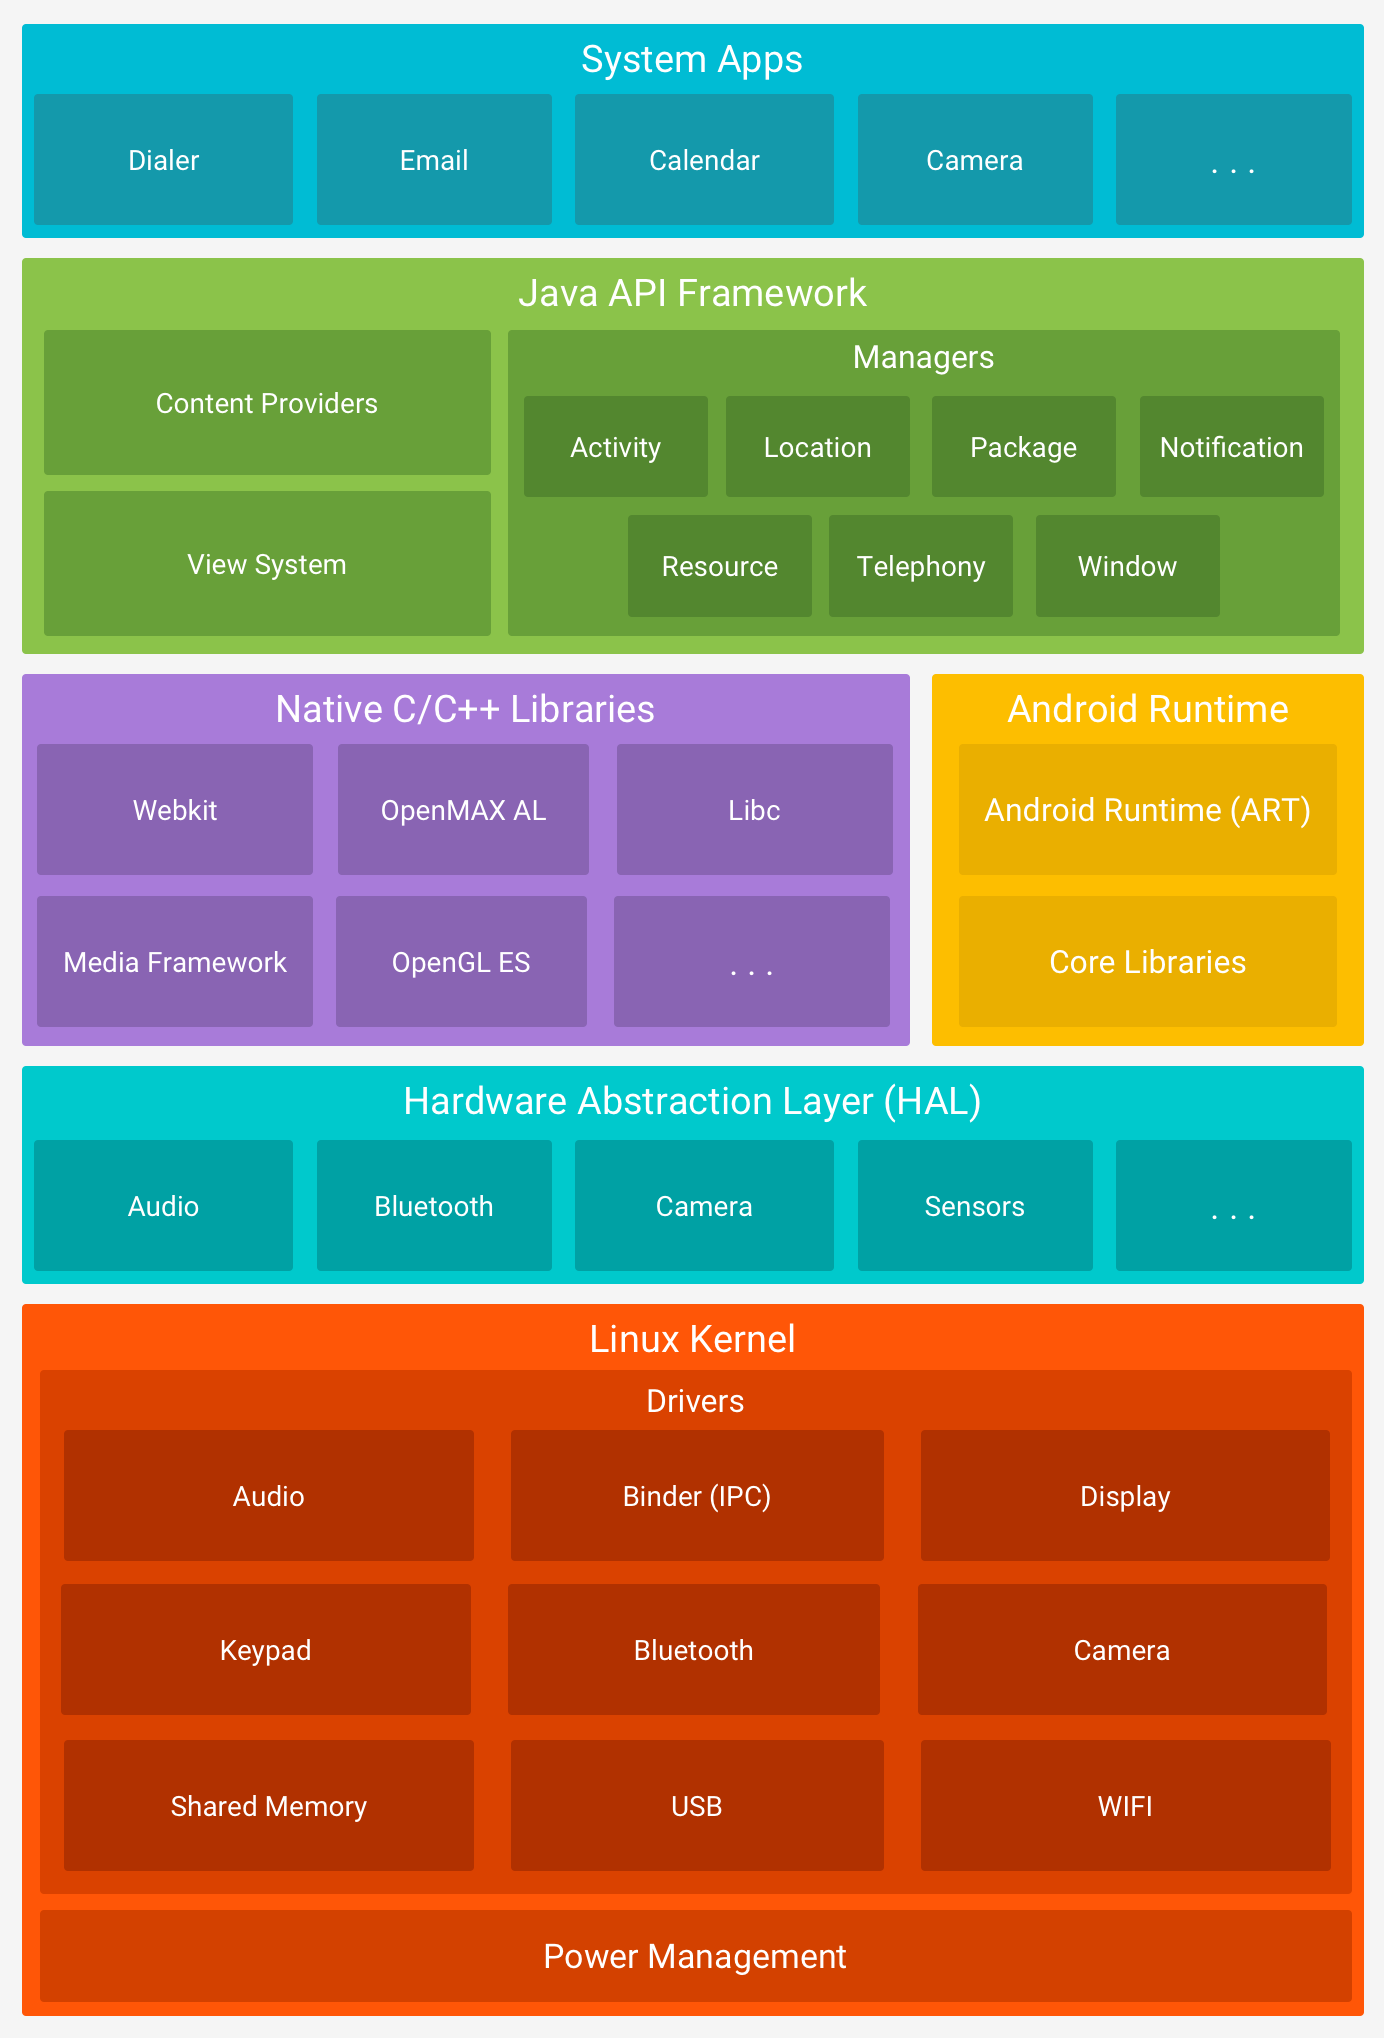
\includegraphics[width=0.7\textwidth]{android-architecture.png}
	\caption{Arquitetura do sistema operacional Android.}
	\label{fig:AndroidPlatform}
\end{figure}

Cada aplicativo � executado em um novo processo de sistema que cont�m sua pr�pria inst�ncia do ambiente de execu��o Android. A partir da vers�o 5 (API n�vel 21), o ambiente de execu��o padr�o � o Android Runtime (ART), antes desta vers�o era a Dalvik. ART foi escrita para executar multiplas inst�ncias de m�quina virtual em dispositivos com pouca mem�ria. Suas funcionalidades incluem duas forma de compila��o: a frente do tempo (AOT do ingl�s \textit{Ahead-of-time}) e apenas no momento (JIT do ingl�s \textit{Just-in-time}), o coletor de lixo, ferramentas de depura��o e um relat�rio de diagn�sticos de erros e exce��es.

Muitos dos componentes e servi�os b�sicos do Android, como ART e HAL, foram criados a partir de c�digo nativo que depende de bibliotecas nativas escritas em C e C++. A plataforma Android prov� arcabou�os de APIs Java para exp�r as funcionalidade de algumas destas bibliotecas nativas para os aplicativos. Por exemplo, OpenGL ES pode ser acessado atrav�s do arcabou�o Android Java OpenGL API, de forma a adicionar suporte ao desenho e manipula��o de gr�ficos 2D e 3D no aplicativo.

Todo as funcionalidades da plataforma Android est�o dispon�veis para os aplicativos atrav�s de APIs Java. Estas APIs comp�em os elementos b�sicos para a constru��o de aplicativos Android. Dentre eles, os mais relevantes para esta disserta��o s�o:

\begin{itemize}
	\item Um rico e extens�vel \textbf{Sistema de Visualiza��o} para a contru��o de interfaces com o usu�rio, tamb�m chamadas de arquivos de \textit{layout}, do aplicativo. Incluindo listas, grades, caixas de textos, bot�es, dentre outros.

	\item Um \textbf{Gerenciador de Recursos}, provendo acesso aos recursos ``n�o-java'' como textos, elementos gr�ficos, arquivos de \textit{layout}.

	\item Um \textbf{Gerenciador de Activity} que gerencia o ciclo de vida dos aplicativos e prov� uma navega��o comum.
\end{itemize}

O Android j� vem com um conjunto de aplicativos b�sicos como por exemplo, para envio e recebimento de SMS, calend�rio, navegador, contatos e outros. Estes aplicativos vindos com a plataforma n�o possuem nenhum diferencial com rela��o aos aplicativos de terceiros. Todo aplicativo tem acesso ao mesmo arcabou�o de APIs do Android, seja ele aplicativo da plataforma ou de terceiro. Desta forma, um aplicativo de terceiro pode se tornar o aplicativo padr�o para navegar na internet, receber e enviar SMS e assim por diante.

Aplicativos da plataforma provem capacidades b�sicas que aplicativos de terceiros podem reutilizar. Por exemplo, se um aplicativo de terceiro quer possibilitar o envio de SMS, o mesmo pode redirecionar esta funcionalidade de forma a abrir o aplicativo de SMS j� existente, ao inv�s de implementar por si s�.

\subsection{Aplicativos Android}

Aplicativos Android s�o escritos na linguagem de programa��o Java. O Kit para Desenvolvimento de Software (SDK do ingl�s \textit{Software Development Kit}) Android compila o c�digo, junto com qualquer arquivo de recurso ou dados, em um arquivo Android Package (APK). Um APK, arquivo com extens�o \texttt{.apk}, � usado por dispositivos para a instala��o de um aplicativo \cite{AndroidFundamentals}.

Componentes Android s�o os elementos base para a constru��o de aplicativos Android. Cada componente � um diferente ponto atrav�s do qual o sistema pode acionar o aplicativo. Nem todos os componente s�o pontos de entrada para o usu�rio e alguns s�o dependentes entre si, mas cada qual existe de forma aut�noma e desempenha um papel espec�fico. 

Existem quatro tipos diferentes de componentes Android. Cada tipo serve um prop�sito distinto e tem diferentes ciclos de vida, que definem como o componente � criado e destru�do. Os quatro componentes s�o:

\begin{itemize}

	\item \textbf{Activities}

	Uma \textit{activity} representa uma tela com uma interface de usu�rio. Por exemplo, um aplicativo de email pode ter uma \textit{activity} para mostrar a lista de emails, outra para redigir um email, outra para ler emails e assim por diante. Embora \textit{activities} trabalhem juntas de forma a criar uma experi�ncia de usu�rio (UX do ingl�s \textit{User Experience}) coesa no aplicativo de emails, cada uma � independente da outra. Desta forma, um aplicativo diferente poderia iniciar qualquer uma destas \textit{activities} (se o aplicativo de emails permitir). Por exemplo, a \textit{activity} de redigir email no aplicativo de emails, poderia solicitar o aplicativo c�mera, de forma a permitir o compartilhamento de alguma foto. Uma \textit{activity} � implementada como uma subclasse de \texttt{Activity}.  

	\item \textbf{Services}

	Um \textit{service} � um componente que � executado em plano de fundo para processar opera��es de longa dura��o ou processar opera��es remotas. Um \textit{service} n�o prov� uma interface com o usu�rio. Por exemplo, um \textit{service} pode tocar uma m�sica em plano de fundo enquanto o usu�rio est� usando um aplicativo diferente, ou ele pode buscar dados em um servidor remoto atrav�s da internet sem bloquear as intera��es do usu�rio com a \textit{activity}. Outros componente, como uma \textit{activity}, podem iniciar um \textit{service} e deix�-lo executar em plano de fundo. � poss�vel interagir com um \textit{service} durante sua execu��o. Um \textit{service} � implementado como uma subclasse de \texttt{Service}.

	\item \textbf{Content Providers}

	Um \textit{content provider} gerencia um conjunto compartilhado de dados do aplicativo. Estes dados podem estar armazenados em arquivos de sistema, banco de dados SQLite, servidor remoto ou qualquer outro local de armazenamento que o aplicativo possa acessar. Atrav�s de \textit{content providers}, outros aplicativos podem consultar ou modificar (se o \textit{content provider} permitir) os dados. Por exemplo, a plataforma Android disponibiliza um \textit{content provider} que gerencia as informa��es dos contatos dos usu�rios. Desta forma, qualquer aplicativo, com as devidas permiss�es, pode consultar parte do \textit{content provider} (como \texttt{ContactsContract.Data}) para ler e escrever informa��es sobre um contato espec�fico. Um \textit{content provider} � implementado como uma subclasse de \texttt{ContentProvider}.

	\item \textbf{Broadcast Receivers}

	Um \textit{broadcast receiver} � um componente que responde a mensagens enviadas pelo sistema. Muitas destas mensagens s�o originadas da plataforma Android, por exemplo, o desligamento da tela, baixo n�vel de bateria e assim por diante. Aplicativos de terceiros tamb�m podem enviar mensagens, por exemplo, informando que alguma opera��o foi conclu�da. No entanto, \textit{broadcast receivers} n�o possuem interface de usu�rio. Para informar o usu�rio que algo ocorreu, \textit{broadcast receivers} podem criar notifica��es. Um \textit{broadcast receiver} � implementado como uma subclasse de \texttt{BroadcastReceiver}.

\end{itemize}

Antes de a plataforma Android poder iniciar qualquer um dos componente supremencionados, a plataforma precisa saber que eles existem. Isso � feito atrav�s da leitura do arquivo \texttt{AndroidManifest.xml} do aplicativo (arquivo de manifesto). Este arquivo deve estar no diret�rio raiz do projeto do aplicativo e deve conter a declara��o de todos os seus componentes.

O arquivo de manifesto � um arquivo XML e pode conter muitas outras informa��es al�m das declara��es dos componentes do aplicativo, por exemplo:

\begin{itemize}
	\item Identificar qualquer permiss�o de usu�rio requerida pelo aplicativo, como acesso a internet, acesso a informa��es de contatos do usu�rio e assim por diante.

	\item Declarar o n�vel m�nimo do Android requerido para o aplicativo, baseado em quais APIs s�o usadas pelo aplicativo.

	\item Declarar quais funcionalidades de sistema ou \textit{hardware} s�o usadas ou requeridas pelo aplicativo, por exemplo c�mera, \textit{bluetooth} e assim por diante.

	\item Declarar outras APIs que s�o necess�rias para uso do aplicativo (al�m do arcabou�o de APIs do Android), como a biblioteca do Google Maps.
\end{itemize}

Os elementos usados no arquivo de manifesto s�o definidos pelo vocabul�rio XML do Android. Por exemplo, uma \textit{activity} pode ser declarada conforme o \textit{listing} \ref{lst:AndroidManifest}. \\

\begin{lstlisting}[
	language=XML, 
	caption={Arquivo \texttt{AndroidManifest.xml}}, 
	label={lst:AndroidManifest}
]
<?xml version="1.0" encoding="utf-8"?>
<manifest ... >
    <application android:icon="@drawable/app_icon.png" ... >
        <activity android:name="com.example.project.ExampleActivity"
                  android:label="@string/example_label" ... >
        </activity>
        ...
    </application>
</manifest>	
\end{lstlisting}

No elemento \texttt{<application>} o atributo \texttt{android:icon} aponta para o �cone, que � um recurso, que identifica o aplicativo. No elemento \texttt{<activity>}, o atributo \texttt{android:name} especifica o nome da classe completamente qualificado de uma subclasse de \texttt{Activity} e o atributo \texttt{android:label} especifica um texto para ser usado como t�tulo da atividade.

Para declarar cada um dos quatro tipos de componentes, deve-se usar os elementos a seguir:
\begin{itemize}
	\item \texttt{<activity>} elemento para \textit{activities}.
	\item \texttt{<service>} elemento para \textit{services}.
	\item \texttt{<receiver>} elemento para \textit{broadcast receivers}.
	\item \texttt{<provider>} elemento para \textit{content providers}.
\end{itemize}

\subsection{Recursos do Aplicativo}

Um aplicativo Android � composto por outros arquivos al�m de c�digo Java, ele requer \textbf{recursos} como imagens, arquivos de �udio, e qualquer recurso relativo a apresenta��o visual do aplicativo \cite{AndroidFundamentals}. Tamb�m � poss�vel definir anima��es, menus, estilos, cores e arquivos de \textit{layout} das \textit{activities}. Recursos costumam ser arquivos XML que usam o vocabul�rio definido pelo Android.

Um dos aspectos mais importantes de prover recursos separados do c�digo-fonte � a habilidade de prover recursos alternativos para diferentes configura��es de dispositivos como por exemplo idioma ou tamanho de tela. Este aspecto se torna mais importante conforme mais dispositivos s�o lan�ados com configura��es diferentes. Segundo levantamento, em 2015 foram encontrados mais de 24 mil dispositivos diferentes com Android \cite{AndroidFragmentation}.

De forma a prover compatibilidade com diferentes configura��es, deve-se organizar os recursos dentro do diret�rio \texttt{res} do projeto, usando sub-diret�rios que agrupam os recursos por tipo e configura��o. Para qualquer tipo de recurso, pode-se especificar uma op��o padr�o e outras alternativas. 

\begin{itemize}
	\item \textbf{Recursos padr�es} s�o aqueles que devem ser usados independente de qualquer configura��o ou quando n�o h� um recurso alternativo que atenda a configura��o atual. Por exemplo, arquivos de \textit{layout} padr�o ficam em \texttt{res/layout}.

	\item \textbf{Recursos alternativos} s�o todos aqueles que foram desenhados para atender a uma configura��o espec�fica. Para especificar que um grupo de recursos � para ser usado em determinada configura��o, basta adicionar um qualificador ao nome do diret�rio. Por exemplo, arquivos de \textit{layout} para quando o dispositivo est� em posi��o de paisagem ficam em res/layout-land
\end{itemize}

O Android ir� aplicar automaticamente o recurso apropriado atrav�s da identifica��o da configura��o corrente do dispositivo com os recursos dispon�veis no aplicativo. Por exemplo, o recurso do tipo \textit{strings} pode conter textos usados nas interfaces do aplicativo. � poss�vel traduzir estes textos em diferentes idiomas e salv�-los em arquivos separados. Desta forma, baseado no qualificador de idioma usado no nome do diret�rio deste tipo de recurso (por exemplo \texttt{res/values-fr} para o idioma fr�nces) e a configura��o de idioma do dispositivo, o Android aplica o conjunto de \textit{strings} mais apropriado.

A seguir s�o listados os tipos de recursos que podem ser utilizados no Android \cite{AndroidResourceType}. Para cada tipo de recurso existe um conjunto de qualificadores que podem ser usados para prover recursos alternativos:

\begin{itemize}
	\item \textbf{Recursos de anima��es} Definem anima��es pr�-determinadas. Ficam nos diret�rios \texttt{res/anim} ou \texttt{res/animator}.

	\item \textbf{Recursos de lista de cores de estado} Definem recursos de cores que alteram baseado no estado da \textit{View}. Ficam no diret�rio \texttt{res/color}.	

	\item \textbf{Recursos de desenhos} Definem recursos gr�ficos com \textit{bitmap} ou XML. Ficam no diret�rio \texttt{res/drawable}.

	\item \textbf{Recursos de \textit{layouts}} Definem a parte visual da interface com o usu�rio. Ficam no diret�rio \texttt{res/layout}.

	\item \textbf{Recursos de menus} Definem os conte�dos dos menus da aplica��o. Ficam no diret�rio \texttt{res/menu}.

	\item \textbf{Recursos de textos} Definem textos, conjunto de textos e plurals. Ficam no diret�rio \texttt{res/values}.

	\item \textbf{Recursos de estilos} Definem os estilos e e formatos para os elementos da interface com usu�rio. Ficam no diret�rio \texttt{res/values}.

	\item \textbf{Outros recursos} Ainda existem outros recursos como inteiros, \textit{booleanos}, dimens�es, dentre outros. Ficam no diret�rio \texttt{res/values}.
\end{itemize}

 
% -*- root: dissertation.tex -*-
% \todo{Colocar sess�o que fala sobre a importancia de maus cheiros, exemplo tirado dos slides da quali: Classes com antipatterns tendem a ter mais altera��es e falhas. [Khomh et al., 2011]}

Aplicativos Android s�o desenvolvidos, em sua maioria, utilizando a linguagem de programa��o Java \cite{AndroidFundamentals}. Deste modo, um prov�vel questionamento �: ``Por que investigar maus cheiros espec�ficos ao Android quando j� existem tantos maus cheiros e boas pr�ticas documentadas para linguagens orientada a objetos como o Java?''. Para responder a esta pergunta temos as seguintes se��es:

\begin{itemize}
  \item A Se��o \ref{android-vs-tradicional} apresenta pesquisas que investigaram e encontraram importantes caracter�sticas que diferenciam projetos Android de projetos de sistemas tradicionais, como projetos web e cliente/servidor. Essas caracter�sticas agregam complexidades ao desenvolvimento Android n�o encontradas no desenvolvimento de sistemas tradicionais. 

  \item A Se��o \ref{maus-cheiros-especificos} apresenta pesquisas que t�m demonstrado que diferentes tecnologias podem apresentar maus cheiros espec�ficos. H� pesquisas que concluem que, tecnologias usadas na camada de apresenta��o de sistemas tradicionais, apresentam maus cheiros espec�ficos. Essas conclus�es refor�am nossa hip�tese de que o desenvolvimento da camada de apresenta��o Android tamb�m pode apresentar maus cheiros espec�ficos.

  \item A Se��o \ref{maus-cheiros-android} apresenta pesquisas que (i) investigaram a presen�a de maus cheiros tradicionais em aplicativos Android, (ii) a exist�ncia de maus cheiro espec�ficos ao Android e tamb�m (iii) compararam a presen�a dos maus cheiros tradicionais com a presen�a de maus cheiros espec�ficos em aplicativos Android. Essas pesquisas refor�am a relev�ncia de investigarmos maus cheiros espec�ficos ao Android pois concluem que maus cheiros espec�ficos aparecem muito mais do que os maus cheiros tradicionais.
\end{itemize}

Ao final desta se��o esclarecemos os motivos pelo qual optamos por investigar maus cheiros de c�digo relacionados � camada de apresenta��o Android e tamb�m darmos uma vis�o s�lida do estado da arte sobre o assunto.

% Muitas pesquisas t�m sido realizadas sobre a plataforma Android, muitas delas focam em vulnerabilidades \cite{Y, F, G, X, P, D, E}, autentica��o \cite{T, Yamashita6405287, R} e testes \cite{J, M}. Diferentemente dessas pesquisas, nossa pesquisa tem foco na percep��o dos desenvolvedores sobre boas e m�s pr�ticas de desenvolvimento na plataforma Android. 

\section{Maus Cheiros Tradicionais}
\todo{Em constru��o.}
% Disserta��o do Aniche e Palomba e Bavota


\section{Projetos Android vs. projetos de sistemas tradicionais}
\label{android-vs-tradicional}

  Minelli e Lanza \cite{Mantyla2013} apresentam diferen�as no desenvolvimento de aplicativos e sistemas tradicionais em termos de m�tricas de c�digo, uso de APIs terceiras e evolu��o. Para isso os autores se utilizam da ferramenta SAMOA, desenvolvida por eles, para realizar a an�lise est�tica de c�digo.

  � interessante que para an�lise do c�digo Android, os autores segmentam o c�digo em dois grupos, ``classes n�cleo'' e ``classes n�o n�cleo'', similar a defini��o usada por Verloop \cite{MobileSmells:13}, onde classes n�cleo est�o relacionadas �s classes que herdam do Android SDK e classes n�o n�cleo seriam todas as outras. Apesar dessa defini��o, Minelli e Lanza \cite{Mantyla2013} coletam quais c�digos ser�o analisados, as classes n�cleo, do arquivo \textit{AndroidManifest.xml}. Por�m, existem diversas classes em um projeto Android, que herdam do Android SDK, e n�o precisam ser declaradas no arquivo \textit{AndroidManifest.xml}, ou seja, a defini��o dos autores abrange muito mais c�digo do que de fato foi analisado na pesquisa.

  Os autores concluem com um conjunto de caracter�sticas de aplicativos Android e com um conjunto de h�bitos dos desenvolvedores destes aplicativos que diferem de aplica��es de sistemas tradicionais. Dentre as caracter�sticas, afirmam que algumas vezes o c�digo n�cleo do app � composto por uma, ou algumas, \textit{God Classes} e que heran�a, para o uso de \textit{design} das classes, � algo quase inexistente em aplicativos Android. Estas constata��es refor�am um mau cheiro por n�s identificado sobre a falta de arquitetura padr�o, visto que esta exige um conhecimento mais aprimorado de orienta��o a objetos.

\section{Maus cheiros espec�ficos a uma tecnologia}
\label{maus-cheiros-especificos}

  A constante e r�pida evolu��o de tecnologias existentes e a cria��o de novas tecnologias faz com que diversos temas, como manutenibilidade de sistemas, estejam tamb�m em constante alta. Muitos pesquisadores v�m pesquisando sobre a exist�ncia de maus cheiros de c�digo espec�ficos a uma dada tecnologia, como por exemplo, arcabou�os Java \cite{MvcSmells:16, ORMSmells}, a linguagem CSS (\textit{Cascading Style Sheets}) \cite{CSSCodeSmell} e f�rmulas em planilhas \cite{SpreadsheetsSmells:12}.

  Chen et al. \cite{ORMSmells} viram a necessidade de estudar maus cheiros de c�digo em arcabou�os de Mapeamento Objeto-Relacional (ORM, do ingl�s \textit{Object-Relational Mapping}) pelo grande uso pela ind�stria e pela desaten��o de desenvolvedores sobre ao impacto de seus c�digos no desempenho do banco de dados que podiam causar estouro no limite de tempo de processamento (``\textit{timeouts}'') e paradas nos sistemas. Os autores implementaram um arcabou�o automatizado e sistem�tico para detectar e priorizar anti-padr�es de desempenho em aplica��es desenvolvidas usando ORM e tamb�m mapearam dois anti-padr�es espec�ficos a arcabou�os ORM.

  Aniche et al. \cite{AnicheSmellsMVC:17, MvcSmells:16, FinavaroAniche2016} investigaram maus cheiros de c�digo relacionado ao arcabou�o Spring MVC, usado para o desenvolvimento da camada de apresenta��o de aplica��es web Java. Os autores encontram maus cheiros espec�ficos a cada camada do arcabou�o Spring MVC, modelo, visualiza��o e controladora, afirmando que cada papel arquitetural possui responsabilidades diferentes o que resulta em distribui��es diferentes de valores de m�trica de c�digo e maus cheiros diferentes. Dentre as principais contribui��es deste trabalho est� um cat�logo com seis maus cheiros espec�ficos ao arcabou�o Spring MVC mapeados e validados.

  Gharachorlu \cite{CSSCodeSmell} investigou maus cheiros em c�digo CSS, linguagem amplamente utilizada na camada de apresenta��o de aplica��es web para separar a sem�ntica de apresenta��o do conte�do HTML. De acordo com o autor, apesar da simplicidade de sintaxe do CSS, as caracter�sticas espec�ficas da linguagem tornam a cria��o e manuten��o de CSS uma tarefa desafiadora. Foi realizando um estudo emp�rico de larga escala onde os resultados indicaram que o CSS de hoje sofre significativamente de padr�es inadequados e est� longe de ser um c�digo bem escrito. Gharachorlu prop�e o primeiro modelo de qualidade de c�digo CSS derivado de uma grande amostra de aprendizagem de modo a ajudar desenvolvedores a obter uma estimativa do n�mero total de cheiros de c�digo em seu c�digo CSS. Sua principal contribui��o foi um conjunto de oito novos maus cheiros CSS detectados com o uso da ferramenta CSSNose, tamb�m implementada e disponibilizada pelo autor.

  Fard e Ali \cite{JavascriptSmells} investigaram maus cheiros de c�digo no Javascript, que � uma flex�vel linguagem de \textit{script} para o desenvolvimento do comportamento do lado do cliente, que faz parte da camada de apresenta��o de aplica��es web. Os autores afirmam que devido a essa flexibilidade, o JavaScript � uma linguagem particularmente desafiadora para escrever e manter c�digo. Um dos desafios citados � que, diferentemente de aplicativos Android, que s�o compilados, o Javascript � interpretado. Isso significa que normalmente n�o h� compilador no ciclo de desenvolvimento para ajudar desenvolvedores a detectar c�digo incorreto ou n�o otimizado. Outro ponto que os autores indicam como problema � a natureza din�mica, fracamente tipificada e ass�ncrona, al�m de outros desafios citados. Os autores prop�em um conjunto de 13 maus cheiros de c�digo JavaScript, sendo 7 maus cheiros tradicionais adaptados para o JavaScript e 6 maus cheiros espec�ficos ao JavaScript derivado da pesquisa. Tamb�m � apresentada uma t�cnica automatizada, chamada JSNOSE, para detectar esses maus cheiros.

  % \todo{adicionar par�grafo sobre smells em planilhas, achar ref}

  Uma interessante rela��o que vemos � que muitas pesquisas buscaram por maus cheiros espec�ficos em tecnologias usadas na camada de apresenta��o de aplica��es web \cite{MvcSmells:16, JavascriptSmells, CSSCodeSmell} o que refor�a nossa hip�tese de que aplicativos Android podem seguir o mesmo comportamento possivelmente apresentando maus cheiros espec�ficos � camada de apresenta��o n�o encontrados necessariamente nos demais c�digos da aplica��o.

\section{Maus cheiros em aplicativos Android}
\label{maus-cheiros-android}

  % como vimos na Se��o anterior X.X.X, que inclusive nos mostrou que � poss�vel identificar maus cheiros no \textit{front-end} de aplica��es de sistemas tradicionais e que estes, por sua vez, s�o diferentes dos maus cheiros encontrados no \textit{back-end}. Outras pesquisas concluem que projetos Android possuem caracter�sticas diferentes de projetos java \cite{Hecht:15, Mannan_Dig_Ahmed_Jensen_Abdullah_Almurshed, 30QualitySmells:14}, como vimos na Se��o X.X.X. 

  % por exemplo, o \textit{front-end} � representado por arquivos XML e o ponto de entrada da aplica��o � dado por \textit{event-handler} \cite{AndroidActivities2016} como o m�todo \textsc{onCreate}. Encontramos tamb�m diversas pesquisas sobre \textit{code smells} sobre tecnologias usadas no desenvolvimento de \textit{front-end} web como CSS \cite{CSSCodeSmell} e JavaScript \cite{BB}. Essas pesquisas nos inspiraram a buscar entender se existem \textit{code smells} no \textit{front-end} Android. \\

  Pesquisas relacionadas a maus cheiros em aplicativos Android ainda s�o poucas. Umme et al. \cite{Mannan_Dig_Ahmed_Jensen_Abdullah_Almurshed} afirmam que, das principais confer�ncias de manuten��o de sistemas, dentre 2008 a 2015, apenas 10\% dos artigos consideraram em suas pesquisas, projetos Android e nenhuma outra plataforma m�vel foi considerada. As confer�ncias consideradas foram as ICSE, FSE, OOPSLA/SPLASH, ASE, ICSM/ICSME, MRS e ESEM. 

  Dentre as pesquisas analisadas para efeitos deste trabalho, podemos classificar em 3 grupos: 1) aquelas que buscam por maus cheiros tradicionais em aplicativos Android, 2) as que buscam por maus cheiros espec�ficos a aplicativos Android, grupo ao qual nossa pesquisa est� inserida, 3) e as que buscam ambos os maus cheiros, espec�ficos e tradicionais, em aplicativos Android e comparam qual deles � mais frequente. 

  As se��es seguintes tratam do estado da arte de cada um desses grupos bem como suas semelhan�as e diferen�as com nossa pesquisa.

  \subsection{Presen�a de maus cheiros tradicionais em aplicativos Android}
    Linares-V�squez et al. \cite{DomainMatters} usaram a ferramenta DECOR para realizar a detec��o de 18 diferentes anti-padr�es orientado a objetos em aplicativos m�veis desenvolvidos com Java Mobile Edition (J2ME) e entender a rela��o dos maus cheiros com o dom�nio de neg�cio e m�tricas de qualidade. Dentre as principais conclus�es do estudo temos que, existe uma grande diferen�a nos valores das m�tricas de qualidade em aplicativos afetados pelos maus cheiros e pelos que n�o s�o, e que enquanto h� maus cheiros presentes em todos os dom�nios, alguns s�o mais presentes em dom�nios espec�ficos. %[\todo{quais as semelhan�as e diferen�as??? reler trabalho e comparar com o meu}]

    Verloop \cite{MobileSmells:13} investigou a presen�a de maus cheiros de c�digos tradicionais propostos por Fowler \cite{Refactoring:99} (\textit{Long Method}, \textit{Large Class}, \textit{Long Parameter List}, \textit{Feature Envy} e \textit{Dead Code}) em aplicativos Android para determinar se esses maus cheiros ocorrem mais frequentemente em \emph{classes n�cleo}, classes no projeto Android que precisam herdar de classes do SDK Android, como por exemplo \textit{Activities}, \textit{Fragments} e \textit{Services}, comparando com classes n�o n�cleo. Para isso, ele fez uso de 4 ferramentas de detec��o autom�tica de maus cheiros: JDeodorant, Checkstyle, PMD e UCDetector.  

    % O desenvolvimento Android � basicamente atrav�s da linguagem Java, considerando isso, uma pergunta �bvia seria: Por que buscar por maus cheiros espec�ficos Android se j� existem tantos definidos aplic�veis a c�digo Java? Uma caracter�stica do Android � que, apesar de ser c�digo Java, muitas classes em projetos Android precisam herdar de classes do SDK Android, por exemplo Activities, Fragments e Services.  Essa caracter�stica o torna diferente e portanto, sucet�vel a apresentar maus cheiros espec�ficos. Verloop classifica todo c�digo Java, em um projeto Android, que precisa herdar de classes do SDK Android como classes n�cleo. Durante sua an�lise, ele compara a presen�a dos maus cheiros em classes n�cleo e n�o n�cleo, sendo esta �ltima, classes puramente Java.

    % \todo{falar das muitas responsabilidades de activities no background de android}.%
    O autor afirma que classes n�cleos tendem a apresentar os maus cheiros \textit{God Class}, \textit{Long Method}, \textit{Switch Statement} e \textit{Type Checking} pela sua natureza de muitas responsabilidades, sendo que a classe mais observada com estes maus cheiros foram \textit{Activities}. Um ponto a se pensar �, se a natureza da Activity � de ter muitas responsabilidades, talvez estejamos analisando-a a partir de um ponto de vista inadequado ao buscarmos por \textit{God Class} ou \textit{Long Method}, visto que sabe-se agora de que estes maus cheiros de fato a afetam, mas que de certa forma, esse � o \textit{modus operandi} normal dela. Chegamos ao ponto que a natureza do Android pode implicar em maus cheiros espec�ficos que tragam outros ponto de vista que respeitem a natureza de aplicativos Android, e proponham uma refatora��o adequada.

    % O que � interessante �, se esta de classes n�cleo, que caracterizam projetos Android (pois sem isso � apenas um projeto Java), ser� que estes maus cheiros tradicionais nos d�o a informa��o necess�ria para refatorar e aumentar a manutenibilidade do c�digo? Pois, se � da natureza da Activity ser assim, talvez as solu��es propostas para refatorar estes maus cheiros n�o se apliquem ao Android. Logo, chegamos ao ponto que a natureza do Android pode implicar em maus cheiros espec�ficos que tragam outras abordagens, que respeitem a natureza de projetos Android, para refatora��o.

    O autor tamb�m conclui que o mau cheiro tradicional \textit{Long Parameter List} � menos prov�vel de aparecer em classes n�cleo pois nessas classes, a maioria dos m�todos s�o sobrecargas de m�todos da classe herdada proveniente do SDK Android, e como para se realizar uma sobrecarga de m�todo � necess�rio seguir a assinatura do m�todo original, este normalmente n�o � afetado por este mau cheiro. Novamente voltamos ao ponto que maus cheiros tradicionais n�o foram pensados considerando a natureza de projetos Android, que neste caso est� relacionada a heran�a de classes n�cleo.


    % [explicar melhor estes resultados - chapter 6]
    Verloop \cite{MobileSmells:13} conclui propondo cinco refatora��es com o objetivo de mitigar o mau cheiro \textit{Long Method} que se apresentou por diversos motivos em \textit{Activities} e \textit{Adapters}. Dentre essas cinco propostas de refatora��o, ele implementou e experimentou tr�s. por�m ap�s as refatora��es, alguns c�digos ainda apresentavam o mau cheiro.

    % , sendo que:

    % \begin{itemize}

    %   \item A primeira, uso do padr�o \texttt{ViewHolder} em \texttt{Adapter}, de fato melhora a qualidade do c�digo, no exemplo do autor, dos 12 \texttt{Adapter} afetados pelo mau cheiro \textit{Long Method}, ap�s a refatora��o apenas 4 continuaram apresentando o mau cheiro. Este padr�o tr�s resultados n�o apenas em manutenibilidade, mas tamb�m em efici�ncia, realizando um consumo melhor de mem�ria, processamento e energia. Por todos estes benef�cios no uso desse padr�o, atualmente o Android SDK j� prov� um componente com esta implementa��o de forma nativa, o componente \textit{RecyclerView} \footnote{https://developer.android.com/reference/android/support/v7/widget/RecyclerView.html}.
    
    %   \item A segunda, uma esp�cie de ViewHolder para \textit{Activities}, objetivava mitigar Long Method, por�m n�o trouxe bons resultados sendo que das 13 \textit{Activities} refatoradas, nenhum deixou de ser afetada pelo Long Method. Dessa forma, o autor conclui que outros n�o trabalhados por meio da refatora��o proposta influenciam na apari��o deste mau cheiro em \textit{Activities}. Estes outros fatores est�o relacionados a \textit{listeners} e classes an�nimas usados para a implementa��o de comportamento dos elementos da camada de apresenta��o pois estes c�digos s�o comumente colocados no m�todo \texttt{onCreate} de Activities.
    
    %   \item A terceira prop�e mitigar o mau cheiro Long Method em Activities trocando a atribui��o de \textit{listeners} feitas com classes an�nimas pelo uso do atributo \texttt{OnClick} no XML de layout respectivo. Os resultados aqui obtidos tamb�m n�o foram muito satisfat�rios pois, das 13 classes refatoradas, 7 ainda apresentaram o mau cheiro devido ao uso de outros \textit{listeners} que n�o o de \textit{click}, que n�o possuem atributos correspondentes no XML de layout. Al�m disso, j� se sabe hoje que o uso de atributos n�o � interessante devido ao acoplamento resultante da \texttt{Activity} com aquele determinado XML dentre outros problemas. Apesar disso, o autor considerou este resultado como positivo. %\todo{explicar e trazer ref}

    % \end{itemize}

    � interessante notar que dentro da defini��o de Verloop \cite{MobileSmells:13} de classes n�cleo, est�o inclu�das classes que herdam de \textit{Services} e todas as demais que herdam de alguma classe do SDK Android, por�m as �nicas classes que apresentaram maus cheiros foram \textit{Activities} e \textit{Adapters}. Como vimos em \ref{sec:Android}, essas classes s�o respons�veis por lidar com a camada de apresenta��o Android, o que refor�a nossa hip�tese de que a camada de apresenta��o Android tende a ser mais problem�tico que o restante dos c�digos da aplica��o e por isso vale a pena ser estudado mais a fundo. 
  
  \subsection{Maus cheiros espec�ficos a aplicativos Android}

    % \todo{explicar mais, com exemplos, do que se tratam os maus cheiros encontrados nesses trabalhos e por que os meus s�o diferentes}

    % \todo{quais?}
    Gottschalk et al. \cite{RemovingEnergySmells:12} conduziram um estudo sobre formas de detectar e refatorar maus cheiros de c�digo relacionados ao uso eficiente de energia. Os autores compilaram um cat�logo com 6 cheiros de c�digo extra�dos de outros trabalhos, e trabalharam sob um trecho de c�digo Android para exemplificar um deles, o \textit{Carregar Recurso Muito Cedo}, quando algum recurso � alocado muito antes de precisar ser utilizado. Essa pesquisa � relacionada � nossa por ambas considerarem a tecnologia Android e se diferenciam pois focamos na busca por maus cheiros de c�digo relacionados manutenibilidade enquanto eles tratam de efici�ncia, conforme conceitos de qualidade de sistemas apresentados da Se��o 2.2.

    Reimann et al. \cite{30QualitySmells:14} correlacionam os conceitos de mau cheiro, qualidade e refatora��o a fim de introduzir o termo mau cheiro de qualidade (do ingl�s \textit{quality smell}). Segundo os autores, um mau cheiro de qualidade � uma estrutura que influencia negativamente requisitos de qualidade espec�ficos, que podem ser resolvidos por refatora��es \cite{Reimann}. Os autores compilaram um cat�logo de 30 cheiros de qualidade para Android. O formato dos cheiros de qualidade incluem: nome, contexto, requisitos de qualidades afetados e descri��o. Esse formato foi baseado nos cat�logos de Brown et al. \cite{AntiPatterns:98} e Fowler \cite{Refactoring:99}. Todo o cat�logo pode ser encontrado online\footnote{http://www.modelrefactoring.org/smell\_catalog} e os mesmos tamb�m foram implementados no arcabou�o Refactory \cite{Reimann}. Os requisitos de qualidade tratados por Reimann et al. \cite{30QualitySmells:14} s�o: centrados no usu�rio (estabilidade, tempo de inicio, conformidade com usu�rio, experi�ncia do usu�rio e acessibilidade), consumo inteligente de recursos de hardware do dispositivo (efici�ncia no uso de energia, processamento e mem�ria) e seguran�a. 

    Reimann et al. \cite{30QualitySmells:14} citam que o problema no desenvolvimento m�vel � que os desenvolvedores est�o cientes dos maus cheiros de qualidade apenas indiretamente, que suas defini��es s�o informais como melhores pr�ticas e discuss�es em f�runs. Continua dizendo que os recursos para encontr�-los s�o distribu�dos pela web e que � dif�cil coletar e analisar todas essas fontes sob um ponto de vista comum e fornecer suporte de ferramentas para desenvolvedores. Os autores derivaram os 30 maus cheiros de boas e m�s pr�ticas documentadas online na documenta��o do Android e de postagens em blogs de desenvolvedores que reportaram suas experi�ncias. 
    % (segundo o paper de Geoffrey Hetch - abaixo).\todo{rever isso aqui}

  \subsection{Presen�a de maus cheiros tradicionais vs. maus cheiros espec�ficos em aplicativos Android}

    Hetch \cite{HetchDetectingAntipatternsAndroidApps:15} utilizou a ferramenta de detec��o de maus cheiros P�prika\footnote{https://github.com/geoffreyhecht/paprika} para identificar 8 maus cheiros, sendo 4 tradicionais (\textit{Blob Class} \cite{AntiPatterns:98}, \textit{Swiss Army Knife} \cite{AntiPatterns:98}, \textit{Complex Class} \cite{Refactoring:99} e \textit{Long Method} \cite{Refactoring:99}) e 4 Android (\textit{Internal Getter/Setter} \cite{30QualitySmells:14}, \textit{No Low Memory Resolver} \cite{30QualitySmells:14}, \textit{Member Ignoring Method} \cite{30QualitySmells:14} e \textit{Leaking Inner Class} \cite{30QualitySmells:14}), em 15 aplica��es Android populares como Facebook, Skype e Twitter. Isso foi poss�vel pois a ferramenta P�prika utiliza o APK para extrair os dados para an�lise e mesmo essas aplica��es n�o sendo de c�digo aberto, o P�prika consegue extrair os dados a partir do instal�vel. Um ponto importante � que apesar do autor utilizar o termo anti-padr�o, ele se baseia em outras pesquisas que definiram os ``anti-padr�es'' por ele analisado como maus cheiros de c�digo. Logo, seguiremos com o termo mau cheiro daqui em diante. Vale considerar que, para se classificar como um anti-padr�o, o item deve atender as duas caracter�sticas mencionadas em \cite{AntiPatterns:98} como abordamos na Se��o \ref{sec:anti-patterns}.

    Hetch \cite{HetchDetectingAntipatternsAndroidApps:15} afirma que os maus cheiros tradicionais s�o t�o frequentes em aplicativos Android como em n�o Android, com exce��o ao \textit{Swiss Army Knife}. Essa afirma��o nos leva a entender que ele teria comparado a presen�a dos maus cheiros tradicionais em sistemas tradicionais com os mesmos maus cheiros em aplicativos Android, entretanto, n�o h� informa��es de como o autor obteve a informa��o da presen�a de maus cheiros em projetos de sistemas tradicionais para compar�-la com o resultado obtido em aplicativos Android. 

    Segundo o autor, \textit{Activities} tendem a ser mais sens�veis ao \textit{Blob Class} \cite{AntiPatterns:98} (muito similar a \textit{God Class} \cite{Riel:96} e \textit{Large Class} \cite{Refactoring:99}), muito similar a conclus�o de Verloop \cite{MobileSmells:13}. Esses resultados refor�am nossa hip�tese de que, c�digos pertencentes � camada de apresenta��o Android, s�o mais propensos a apresentar trechos de c�digos problem�ticos. Ainda segundo o autor, maus cheiros espec�ficos Android s�o muito mais frequentes do que os maus cheiros tradicionais. Essa constata��o refor�a a import�ncia de se investigar quais seriam outros poss�veis maus cheiros espec�ficos de forma que eles tendem a se manifestar mais do que os maus cheiros tradicionais.

    

% \section{Android}
% geral android (opcional)
% Na pr�tica, n�o acho que faz sentido pois n�o tenho muito comparar meu trabalho eu acho, mas deixa como opcional

% \section{Maus cheiros espec�ficos ao Android}

%   \subsection{Removing Energy Code Smells with Reengineering Services}

%     Gottschalk et al \cite{RemovingEnergySmells:12} conduziram um estudo sobre formas de detectar e refatorar cheiros de c�digo relacionados ao uso eficiente de energia. Os autores compilaram um cat�logo com 6 cheiros de c�digo extra�do de outros trabalhos, e trabalharam sob um trecho de c�digo Android para exemplificar um deles, o \textit{Carregar Recurso Muito Cedo}, quando algum recurso � alocado muito antes de precisar ser utilizado. Essa pesquisa � relacionada � nossa por ambas considerarem a tecnologia Android e se diferenciam pois focamos na busca por maus cheiros de c�digo relacionados manutenibilidade enquanto eles tratam de efici�ncia, conforme conceitos de qualidade de sistemas apresentados da Se��o 2.2.

%   \subsection{A Tool-Supported Quality Smell Catalogue For Android Developers - Reimann et al.}

%     Reimann et al. \cite{30QualitySmells:14} correlaciona os conceitos de mau cheiro, qualidade e refatora��o a fim de introduzir o termo cheiro de qualidade (do ingl�s \textit{quality smell}). Um cheiro de qualidade � uma estrutura que influencia negativamente requisitos de qualidade espec�ficos, que podem ser resolvidos por refatora��es \cite{Reimann}.

%     Os autores compilaram um cat�logo de 30 cheiros de qualidade para Android. O formato dos cheiros de qualidade incluem: nome, contexto, requisitos de qualidades afetados e descri��o, este formato foi baseado nos cat�logos de Brown et al. \cite{AntiPatterns:98} e Fowler \cite{Refactoring:99}. Todo o cat�logo pode ser encontrado em [http://www.modelrefactoring.org/smell\_catalog](http://www.modelrefactoring.org/smell\_catalog) e os mesmos tamb�m foram implementados no framework Refactory \cite{Reimann}.

%     O requisitos de qualidade tratados por \cite{30QualitySmells:14} s�o: centrados no usu�rio (estabilidade, tempo de inicio, conformidade com usu�rio, experi�ncia do usu�rio e acessibilidade), consumo inteligente de recursos de hardware do dispositivo (efici�ncia no uso de energia, processamento e mem�ria) e seguran�a.

%     Reimann et al. \cite{30QualitySmells:14} cita que o problema no desenvolvimento m�vel � que os desenvolvedores est�o cientes de cheiros de qualidade apenas indiretamente porque suas defini��es s�o informais (melhores pr�ticas, problemas de rastreamento de bugs, discuss�es de f�rum etc.) e os recursos onde encontr�-los s�o distribu�dos pela web e que � dif�cil coletar e analisar todas essas fontes sob um ponto de vista comum e fornecer suporte de ferramentas para desenvolvedores. 

%     Derivou os 30 maus cheiros de boas e m�s pr�ticas documentadas online na documenta��o do Android e de postagens em blogs de desenvolvedores que reportaram suas experi�ncias. (segundo o paper de Geoffrey Hetch - abaixo)


% \section{Presen�a de maus cheiros em projetos Android}

%   \subsection{Code Smells in the Mobile Applications Domain - Verloop}Long Method em Activities trocando atribui��o de listener feitas com classes an�nimas pelo uso do atributo OnClick no layout respectivo. Os resultados aqui obtidos n�o foram muito satisfat�rios tamb�m pois, das 13 classes refatoradas, 7 ainda apresentaram o mau cheiro devido ao uso de outros listeners que n�o o de click, que n�o possuem atributos correspondentes. Al�m disso, j� se sabe hoje que o uso de atributos n�o � interessante devido ao acoplamento resultante da Activity com aquele determiado XML dentre outros problemas [quais?]. Apesar disso, Verloop considerou os resultados bons.

%     � interessante notar que dentro da defini��o de classes n�cleo est�o inclu�das classes que heram de Services, dentre outras, por�m as �nicas classes que apresentaram maus cheiros foram Activities e Adapters. Como vimos em BACKGROUND ANDROID, essas classes s�o respons�veis por lidar com a UI e estes resultados de Verloop refor�am nossa hip�tese que o front-end Android tende a ser mais problem�tico que o restante dos c�digos da aplica��o e por isso vale a pena ser estudado mais a fundo. 
   
%   \subsection{An Approach to Detect Android Antipatterns - Geoffrey HetcLongo [12]) e 4 Android (Internal Getter/Setter, No Low Memory Resolver, Member Ignoring Method e Leaking Inner Class), definidos por [Reimann] em 15 aplica��es Android populares como Facebook, Skype, Twitter. Isso foi poss�vel pois a ferramenta P�prika se utiliza do APK para extrair os dados para an�lise. Um ponto importante � que apesar de Hetch utilizar do termo anti-patterns, ele se baseia em outros artigos que definiram os \textit{``antipatterns''} por ele analisado como maus cheiros. Logo, seguiremos com o termos mau cheiro, pois entendemos que apesar da diverg�ncia do termo, o autor se refere a ele. Vale considerar que, para se classificar como um antipattern o item deve atender as 2 (ou 3?) caracter�sticas mencionadas em [ref p/ livro de antipatterns] como abordamos na Se��o X.X.X [sobre antipatterns] e n�o h� evid�ncias que de que os itens tratados por Hetch atendem as caracter�sticas mencionadas.

%     Hetch afirma que os maus cheiros tradicionais s�o t�o frequentes em aplicativos Android como em n�o Android, com exce��o ao Swiss Army Knife, mas n�o h� evid�ncias de ele ter executado o P�prika em busca dos mesmos maus cheiros em projetos n�o Android. Segundo o artigo, Activities tendem a ser mais sens�veis ao Blob Class, mau cheiro este muito similar a God Class e Large Class, tamb�m identificado como muito comum por Verloop [?], esta conclus�o refor�a nossa hip�tese que c�digos pertencentes ao front-end Android s�o mais propensos a apresentar trechos problem�ticos, que, apesar de j� existirem maus cheiros que os identificam, a refatora��o proposta n�o � apropriada pois � da natureza de projetos Android apresentarem estes problemas, isso nos leva a pensar que essas situa��es em s� n�o s�o o problema de fato, e que talvez existam outras formas de definir e lidar com esses problemas no Android.

%     Outra conclus�o interessante � que o artigo diz que maus cheiros espec�ficos Android s�o muito mais frequentes do que os maus cheiros tradicionais, o que reafirma a necessidade de pesquisar se h� outros maus cheiros espec�ficos, que tendem tamb�m a ser mais frequentes.

  % \subsection{Detecting antipatterns in Android aplicativos - Geoffrey Hetch}
  %   ???

  % \subsection{Domain Matters: Bringing Further Evidence of the Relatonships among Anti-patterns, Application Domains, and Quality-Related Metrics in Java Mobile aplicativos - Linares-V�squez et al.}

    % Linares-V�squez et al. \cite{DomainMatters} usou a ferramenta DECOR para realizar a detec��o de 18 diferentes \textit{anti-patterns} orientado a objetos em aplicativos m�veis desenvolvidos com Java Mobile Edition (J2ME). Este estudo em larga escala mostra que a presen�a de antipatterns afeta negativamente as m�tricas de qualidade do sistemas, em particular as m�tricas relacionadas � falha.


% \section{aplicativos Android vs. sistemas Tradicional}

%   \subsection{sistemas analytics for mobile applications, insights \& lessons learned - Minelli e Lanza}

%     Os autores apresentam diferen�as no desenvolvimento de aplicativos e sistemas tradicionais em termos de m�tricas de c�digo, uso de APIs terceiras e evolu��o. Para isso se utilizam da ferramenta SAMOA de an�lise est�tica de c�digo desenvolvida por eles.

%     � interessante que para an�lise do c�digo Android eles tamb�m modelam o projeto em c�digo core e n�o core, onde o c�digo core est� relacionado a classes que herdam do Android SDK, apesar disso, eles dizem coletar essa informa��o do Android Manifesto, considerando Activities e Services, entretanto, existem diversas outras classes em um projeto Android que herdam do Android SDK e n�o precisam ser declaradas no Android Manifesto, ou seja, a defini��o usada abrange muito mais c�digo do que de fato analisado pela pesquisa.

%     Concluem com um conjunto de caracter�sticas de aplicativos e com um conjunto de h�bitos dos desenvolvedores destes aplicativos que diferem de aplica��es de sistemas tradicionais. Dentre as caracter�sticas, afirmam que algumas vezes core code do app � composto por uma, ou algumas, God Classes. E que heran�a � algo quase inexistente em aplicativos Android. O que refor�a nossa identifica��o de falta de arquitetura padr�o, visto que esta exige um conhecimento mais aprimorado de orienta��o a objetos que inclui heran�a.

Podemos notar algumas semelhan�as nos trabalhos acima citados. A primeira semelhan�a importante � que diversas pesquisas que analisam a presen�a de maus cheiros, sejam tradicionais ou espec�ficos ao Android, sentem a necessidade de delimitar o c�digo a ser analisado. Podemos observar isso nos trabalhos de Verloop \cite{MobileSmells:13} e Minelli e Lanza \cite{Mantyla2013} atrav�s do termo \emph{classes/c�digos n�cleos} onde, em ambas as pesquisas, significam \emph{classes que herdam do SDK Android}. Essa delimita��o exclui todo o c�digo puramente Java existente no projeto Android, chamado pelos autores de \emph{classes n�o n�cleo}, que s�o classes Java tradicionais, pelo qual continua sendo poss�vel a utiliza��o de diversas boas pr�ticas j� existentes na literatura. 

Ainda com rela��o � delimita��o do c�digo em estudo, outra semelhan�a interessante � que, apesar de a defini��o de classes n�cleo incluir classes como \textit{Services}, \textit{AsyncTasks} dentre muitas outras existentes no SDK Android, as classes que apareceram nos resultados se limitaram a \textit{Activities} e \textit{Adapters}, ambas classes utilizadas para a constru��o e resposta a eventos da camada de apresenta��o Android. 

Essas semelhan�as refor�aram nosso intuito de focar nossa pesquisa no c�digo relacionado � camada de apresenta��o Android, partindo da hip�tese de que existem maus cheiros espec�ficos a ela. De modo que pretendemos pela primeira vez catalogar maus cheiros de c�digo, relacionados � manutenibilidade, especificamente relacionados � camada de apresenta��o de aplicativos do Android.


% Boa frase, s� falta refs e colocar no lugar certo, talvez um bom local seja na descri��o do m�todo de pesquisa
% A percep��o desempenha um importante papel na defini��o de maus cheiros de c�digo relacionados a uma tecnologia, visto que maus cheiros possuem uma natureza subjetiva. Maus cheiros desempenham um importante papel na busca por qualidade de c�digo, visto que, ap�s mapeados, podemos chegar a heur�sticas para identific�-los e com essas heur�sticas, implementar ferramentas que automatizem o processo de identificar c�digos problem�ticos.
% -*- root: dissertacao.tex -*-
%%%%%%%%%%%%%%%%%%%%%%%%%%%%%%%%%%%%%%%%%%%%%%%%%%%%%%%%%%%%%%%%%%%%%%%
\setlength{\parindent}{20pt}
\setlength{\textheight}{22cm}
\setlength{\parskip}{0.2cm}
\linespread{1.2} % Para aumentar o espa�amento entre as linhas
%%%%%%%%%%%%%%%%%%%%%%%%%%%%%%%%%%%%%%%%%%%%%%%%%%%%%%%%%%%%%%%%%%%%%%%

\chapter{Camada de Apresenta��o Android}
\label{ch:PresentationLayer}

Um assunto essencial para o entendimento deste trabalho � explanar o que queremos dizer com ``Camada de Apresenta��o Android''. Nesta se��o abordamos justamente este assunto de forma a explanar como chegamos na defini��o aqui usada.

Em nossas pesquisas bibliogr�ficas n�o foi econtrada uma defini��o formal sobre camada de apresenta��o Android. Encontramos por�m, pontos na documenta��o oficial do Android \cite{AndroidDeveloperSite2016} que afirmam que determinado elemento de alguma forma � parte desta camada. Por exemplo o trecho sobre \textit{Activities} diz que ``representa uma tela com interface do usu�rio''. O trecho sobre recursos do aplicativo afirma que ``um aplicativo Android � composto por outros arquivos al�m de c�digo Java, ele requer recursos como imagens, arquivos de �udio e qualquer recurso relativo a apresenta��o visual do aplicativo'' \cite{AndroidFundamentals}. Encontramos tamb�m postagens em sites t�cnicos sobre Android que de alguma forma indicam que determinado elemento comp�e a camada de apresenta��o Android, por exemplo Preussler relaciona \textit{adapters} como parte da camada de apresenta��o \cite{AdaptersPreussler2016}. Desta forma viu-se necess�rio definir quais s�o os elementos, para efeitos desta disserta��o, que comp�em a camada de apresenta��o em aplicativos Android. 

Os prim�rdios de GUI (\textit{Graphical User Interfaces} ou Interfaces de Usu�rio Gr�ficas) foram em 1973 com o projeto Alto, desenvolvido pelos pesquisadores da Xerox Palo Alto Research Center (PARC), seguido do projeto Lisa da Apple em 1979. Estes dois projetos serviram de base e inspira��o para o Machintosh, lan�ado pela Apple em 1985. As primeiras defini��es sobre GUI que surgiram nessa �poca abordavam sobre componentes de uso comum como �cones, janelas, barras de rolagem, menus supensos, bot�es, caixas de entrada de texto; gerenciadores de janelas; arquivos de �udio, internacionaliza��o e eventos. Antes deste per�odo existiam apenas interfaces de linha de comando \cite{GUIRaymond2004, UITecMundo2016}.

Outra fonte define camada de apresenta��o como ``informa��es gr�ficas, textuais e auditivas apresentadas ao utilizador, e as sequ�ncias de controle (como comandos de teclado, \textit{mouse} ou toque) para interagir com o programa'' \cite{UIWikipedia2016}. 

Unindo as defini��es supracitadas, definimos que todos os elementos do Android que s�o apresentados ou interagem com o usu�rio de alguma forma auditiva, visual ou por comando de voz ou toque s�o elementos da \textbf{Camada de Apresenta��o}, s�o eles:

\begin{itemize}
	\item \textbf{Activities e Fragments} Representam uma tela ou um fragmento de tela. A exemplo temos classes Java que herdam de \texttt{Activity}, \texttt{Fragment} ou classes similares.

	\item \textbf{Listeners} Meio pelo qual os comandos do usu�rio s�o capturados pelo aplicativo. A exemplo temos classes Java que implementam interfaces como \texttt{View.OnClickListener}.

	\item \textbf{Recursos do Aplicativo} Arquivos que apresentam textos, imagens, �udios, menus, interfaces gr�ficas (\textit{layout}), dentre outros. Est�o inclu�dos neste item todos os arquivos dentro do diret�rio \texttt{res} ainda que em seu formato Java. A exemplo podemos citar classes que herdam da classe \texttt{View} ou \texttt{ViewGroup}.

	\item \textbf{Adapters} Meio pelo qual s�o carregados conte�dos din�micos ou n�o pr�-determinados na tela. A exemplo podemos citar classes que herdam da classe \texttt{BaseAdapter}.

\end{itemize}


% -*- root: dissertacao.tex -*-
%%%%%%%%%%%%%%%%%%%%%%%%%%%%%%%%%%%%%%%%%%%%%%%%%%%%%%%%%%%%%%%%%%%%%%%
\setlength{\parindent}{20pt}
\setlength{\textheight}{22cm}
\setlength{\parskip}{0.2cm}
\linespread{1.2} % Para aumentar o espa�amento entre as linhas
%%%%%%%%%%%%%%%%%%%%%%%%%%%%%%%%%%%%%%%%%%%%%%%%%%%%%%%%%%%%%%%%%%%%%%%

\chapter{Proposta de Disserta��o}

Conforme apresentado no Cap�tulo 1, podem existir maus cheiros espec�ficos a um dom�nio, tecnologia ou plataforma (por exemplo, Android) \cite{FinavaroAniche2016, DomainMatters, MobileSmells:13}. Geoffrey \cite{Hecht2015} afirma que a detec��o e especifica��o de padr�es m�veis ainda � um problema em aberto e que \textit{antipatterns} Android s�o mais frequentes em projetos m�veis do que \textit{antipatterns} orientado a objetos. Pesquisas em torno de projetos de aplicativos m�veis ainda s�o poucas \cite{Mannan_Dig_Ahmed_Jensen_Abdullah_Almurshed}. Desta forma, neste cap�tulo � apresentada a proposta da disserta��o e o cronograma de atividades planejadas. 


\section{Atividades}

Para obter as ideias iniciais para a deriva��o dos maus cheiros na camada de apresenta��o Android, foi aplicado um question�rio sobre boas e m�s pr�ticas Android na comunidade de desenvolvedores do Brasil e exterior. O question�rio pode ser encontrado no Ap�ndice A e at� o momento da escrita desta proposta de qualifica��o foram coletadas 44 respostas. Ainda de modo a complementar os dados coletados com o question�rio, pretende-se realizar entrevista com desenvolvedores Android sobre o mesmo tema. Tamb�m ser� feito uma an�lise para derivar os maus cheiros, essa an�lise ser� feita com base em estrat�gias j� utilizadas em trabalhos anteriores como o de Aniche et al. \cite{FinavaroAniche2016}. Para reduzir vi�s sobre os maus cheiros definidos, os mesmos ser�o validados com mais de um especialista em Android. A deriva��o dos maus cheiros est� relacionada a Q1 definida na se��o 1.1 e as atividades planejadas s�o:

\begin{itemize} 
	\item Bibliografia e Trabalhos Relacionados.
	\item Survey Boas e M�s pr�ticas Android.
	\item Deriva��o dos Maus Cheiros.
	\item Valida��o Maus Cheiros c/ Especialista.
\end{itemize}

Evid�ncias na literatura sugerem que maus cheiros de c�digo podem esconder manutenibilidade de c�digo \cite{Sjoberg_Quantifying_2013, Yamashita6405287, Yamashita:2013:EII:2486788.2486878} e aumentar a tend�ncia a mudan�as e introdu��o de defeitos \cite{Khomh:2009:ESI:1685994.1686210, Khomh:2012:ESI:2158916.2158921}. Mario et al. \cite{DomainMatters} mostra que \textit{antipatterns} impactam negativamente m�tricas relacionadas a qualidade em projetos m�veis, em particular m�tricas relacionadas a propens�o de falhas. Desta forma, pretende-se avaliar o impacto dos maus cheiros propostos na tend�ncia a mudan�as e introdu��o de defeitos no c�digo. Para isso ser� realizado um experimento presencial com desenvolvedores Android. Este experimento est� relacionado ao Q2 definida na Se��o 1.1 e a atividade planejada �:

\begin{itemize} 
	\item Experimento Impacto em Mudan�as/Defeitos.
\end{itemize}

Evid�ncias na literatura tamb�m sugerem que maus cheiros de c�digo s�o percebidos por desenvolvedores \cite{Palomba_Do_2014}, desta forma pretende-se avaliar se desenvolvedores Android percebem c�digos afetados pelos maus cheiros propostos como indicativos de trechos de c�digos ruins. Para isso ser� conduzido outro experimento tamb�m com desenvolvedores Android. Esse experimento est� relacionado a Q3 definida na Se��o 1.1 e a seguinte atividade est� planejada:

\begin{itemize} 
	\item Experimento Percep��o Desenvolvedores.
\end{itemize}


\section{Cronograma}

Na Tabela \ref{tab:Cronograma} s�o apresentadas as atividades previstas para a conclus�o da disserta��o bem como em qual per�odo pretende-se realiz�-la.

\begin{table}[h]
\centering

\newcommand\T{\rule{0pt}{2.6ex}}       % Top strut
\newcommand\B{\rule[-1.2ex]{0pt}{0pt}} % Bottom strut

\begin{tabular}{|l|cc|cccc|} 
\hline
\multicolumn{1}{|c|}{} 	& \multicolumn{2}{c|}{2016}   	& \multicolumn{4}{c|}{2017} \\
\textbf{Atividades}		& 3$^o$ Tri & 4$^o$ Tri 		& 1$^o$ Tri & 2$^o$ Tri & 3$^o$ Tri & 4$^o$ Tri \\
\hline
\hline
% \rule{0pt}{-1em} 		& 			& 					& 			& 			&			&			\\
Bibliografia e Trabalhos Relacionados 	& \textbullet 	& \textbullet	& 				& 				& 				& 				\T \\
Survey Boas e M�s pr�ticas Android 		& 				& \textbullet	& 				& 				& 				& 				\\
Entrevista Boas e M�s pr�ticas Android	& 				& 				& \textbullet	& 				& 				& 				\\
Deriva��o dos Maus Cheiros 				& 				& 				& \textbullet	& 				& 				& 				\\
Valida��o Maus Cheiros c/ Especialista	& 				& 				& \textbullet	& 				& 				& 				\\
Experimento Impacto em Mudan�as/Defeitos	& 				& 				& 				& \textbullet	& 				& 				\\
Experimento Percep��o Desenvolvedores	& 				& 				& 				& \textbullet 	& 				& 				\\
Escrita da Disserta��o					& \textbullet	& \textbullet	& \textbullet	& \textbullet	& \textbullet	& \textbullet	\\
Defesa									& 				& 				& 				& 				& 				& \textbullet	\B \\
\hline
\end{tabular}
\caption{Cronograma de atividades propostas.}
\label{tab:Cronograma}
\end{table} 
% -*- root: dissertacao.tex -*-
%%%%%%%%%%%%%%%%%%%%%%%%%%%%%%%%%%%%%%%%%%%%%%%%%%%%%%%%%%%%%%%%%%%%%%%
\setlength{\parindent}{20pt}
\setlength{\textheight}{22cm}
\setlength{\parskip}{0.2cm}
\linespread{1.2} % Para aumentar o espa�amento entre as linhas
%%%%%%%%%%%%%%%%%%%%%%%%%%%%%%%%%%%%%%%%%%%%%%%%%%%%%%%%%%%%%%%%%%%%%%%

\chapter{Boas e M�s Pr�ticas na Camada de Apresenta��o}
\label{ch:research}
\label{sc:CodeSmellsDefinition}

Neste cap�tulo � abordado detalhes dos m�todos de pesquisa utilizados para a descoberta dos maus cheiros na camada de apresenta��o Android.


\section{Introdu��o}

\textit{God Class}, \textit{Large Class}, \textit{Long Method} s�o exemplos de maus cheiros de c�digo amplamente reconhecidos por desenvolvedores. De fato, � poss�vel obter m�tricas de qualidade de c�digo de projetos Android utilizando estes maus cheiros j� catalogados. No entanto, pesquisas tem demonstrado que existem maus cheiros de c�digo espec�ficos a tecnologias, frameworks e plataformas \cite{FinavaroAniche2016}, desta forma sugerimos que h� maus cheiros espec�ficos � camada de apresenta��o de aplicativos Android. Para iniciar nossas investiga��es sobre este tema, fizemos a seguinte pergunta:

\begin{center}
\textbf{Q1: O que desenvolvedores consideram boas e m�s pr�ticas com rela��o � Camada de Apresenta��o em projetos Android?}
\end{center}

Maus cheiros de c�digo s�o padr�es de c�digo que est�o associados com um design ruim e m�s pr�ticas de programa��o \cite{MobileSmells:13}. Por si s�, um mau cheiro n�o � algo ruim, ocorre que frequentemente ele indica um problema mas n�o necess�riamente � o problema em si \cite{CodeSmell:06}. Sendo assim, esta quest�o visa identificar quais pr�ticas desenvolvedores Android reconhecem como sendo m�s pr�ticas, e poss�velmente maus cheiros, e quais pr�ticas os desenvolvedores reconhecem como boas pr�ticas, e poss�velmente formas de refatorar o que foi considerado um mau cheiro.

Neste cap�tulo n�s apresentamos um cat�logo de maus cheiros na camada de apresenta��o de projetos Android. Para derivar este cat�logo aplicamos um question�rio respondido por 45 desenvolvedores Android e pretendemos entrevistar outros desenvolvedores sobre boas e m�s pr�ticas seguidas durante o desenvolvimento de aplicativos Android. Tamb�m iremos coletar postagens relacionadas a boas e m�s pr�ticas em sites sobre Android. Ap�s, iremos realizar um procedimento de c�digo aberto a partir das respostas e postagens obtidas. 

Por fim, pretendemos validar os maus cheiros derivados com 2 desenvolvedores especialistas em Android. 

\section{M�todo}

N�s coletamos boas e m�s pr�ticas na camada de apresenta��o seguidas por desenvolvedores durante o desenvolvimento de aplicativos Android. A coleta de dados inclui tr�s diferentes passos, s�o eles:

\textbf{Passo 1: Question�rio Online.} Elaboramos um question�rio em ingl�s com perguntas dissertativas. O question�rio foi divulgado em comunidades de desenvolvedores Android do Brasil e exterior e em redes sociais como LinkedIn, Google Plus, Facebook e Twitter. De forma a obtermos alguma an�lise demogr�fica, as primeiras quest�es questionavam sobre idade e pa�s de resid�ncia.

Em seguida, perguntamos sobre boas e m�s pr�ticas. Para cada elemento da camada de apresenta��o fizemos o seguinte par de perguntas, onde ``X'' indica o elemento da camada de apresenta��o em quest�o: 

\begin{itemize}
	\item Do you have any good practices to deal with X? (Voc� conhece algumas boas pr�ticas para lidar com X?)
	\item Do you have anything you consider a bad practice when dealing whit X? (Voc� considera algo uma m� pr�tica para lidar com X?)
\end{itemize}

Os elementos questionados foram definidos no cap�tulo \ref{ch:PresentationLayer}, s�o eles: \textsc{Activities}, \textsc{Fragments}, \textsc{Adapter}, \textsc{Listeners}, \textsc{layouts}, \textsc{styles}, \textsc{string} e \textsc{drawables}. Os 4 �ltimos representam os 4 principais recursos de aplicativos Android. Optamos por n�o questionar todos os tipos de recursos individualmente para n�o tornar o question�rio muito extenso. 

Por �ltimo, com o objetivo de capturar alguma outra boa ou m� pr�tica em qualquer outro elemento da camada de apresenta��o, adicionamos as seguintes perguntas:

\begin{itemize}
	\item Are there any other *GOOD* practices in Android Presentation Layer we did not asked you or you did not said yet? (Existe alguma outra *BOA* pr�tica na camada de apresenta��o que n�s n�o perguntamos a voc� ou que voc� ainda n�o mencionou?)
	\item Are there any other *BAD* practices in Android Presentation Layer we did not asked you or you did not said yet? (Existe alguma outra *M�* pr�tica na camada de apresenta��o que n�s n�o perguntamos a voc� ou que voc� ainda n�o mencionou?)
\end{itemize}

O question�rio completo pode ser encontrado no ap�ndice 1. \\ 

\textbf{Passo 2: Entrevistas Semi-Extruturadas.} Realizaremos entrevistas semi-estruturadas com desenvolvedores Android. O objetivo da entrevista � fazer com que os desenvolvedores discutam sobre boas e m�s pr�ticas na camada de apresenta��o Android usadas no dia-a-dia de desenvolvimento. Estas discuss�es ser�o focadas nos 8 elementos da camada de apresenta��o questionados no passo anterior. \\ 

\textbf{Passo 3: Pesquisa Bibliogr�fica em Sites T�cnicos.} Realizaremos uma busca na internet por postagens t�cnicas sobre Android que apontem alguma boa ou m� pr�tica em algum dos elementos da camada de apresentac�o pesquisados nos passos anteriores. \\ 

De forma a complementar os dados para an�lise demogr�fica, tanto no question�rio quanto na entrevista fizemos perguntas sobre a experi�ncia com desenvolvimento de software, experi�ncia com desenvolvimento de aplicativos Android nativos e quais linguagens de programa��o se consideravam proeficientes.


\section{Q1: Cat�logo Resultante de Maus Cheiros da Camada de Apresenta��o Android} 



\chapter{Impacto na Tend�ncia a Mudan�as e Defeitos}
\label{sc:ChangeProneness}

\section{Introdu��o}
Evidencias na literatura sugerem que maus cheiros de c�digo podem esconder manutenabilidade de c�digo e aumentar a tend�ncia a mudan�as e introdu��o de defeitos. Neste cap�tulo pretendemos avaliar o impacto dos maus cheiros propostos na tend�ncia a mudan�as e introdu��o de defeitos no c�digo. Para isso conduziremos um experimento presencial com desenvolvedores Android.

\section{M�todo}
Pretende-se conduzir um experimento apresentando aos desenvolvedores um projeto Android onde alguns deles receber�o este projeto com os maus cheiros e outros o receberam com o c�digo j� refatorado. 

Ser� solicitado a todos que implementem uma mesma funcionalidade, esta do qual, necessitar� alterar arquivos da camada de apresenta��o. Com este experimento pretendemos validar o impacto que os maus cheiros propostos tem na tend�ncia a altera��o de c�digo e a introdu��o de defeitos.


\section{Q2: Qual o impacto dos maus cheiros propostos na tend�ncia a mudan�as e defeitos?}

\chapter{Percep��o dos Desenvolvedores}
\label{sc:DevPerceptions}

\section{Introdu��o}
Ap�s a defini��o de um cat�logo de maus cheiros, pretende-se validar se desenvolvedores os percebem de fato como indicativos de trechos de c�digos ruins. Para isso pretende-se conduzir um experimento apresentando aos desenvolvedores c�digos com e sem os maus cheios propostos, para cada c�digo, ser� solicitado que ele indique o c�digo como ``com cheiro'' ou ``sem cheiro''. 

\section{M�todo}

\section{Q3: Os Desenvolvedores percebem os c�digos afetados pelos maus cheiros propostos como problem�ticos?}
 
% % -*- root: dissertacao.tex -*-
%%%%%%%%%%%%%%%%%%%%%%%%%%%%%%%%%%%%%%%%%%%%%%%%%%%%%%%%%%%%%%%%%%%%%%%
\setlength{\parindent}{20pt}
\setlength{\textheight}{22cm}
\setlength{\parskip}{0.2cm}
\linespread{1.2} % Para aumentar o espa�amento entre as linhas
%%%%%%%%%%%%%%%%%%%%%%%%%%%%%%%%%%%%%%%%%%%%%%%%%%%%%%%%%%%%%%%%%%%%%%%

\chapter{Cat�logo de Maus Cheiros}

\section{Code Smell 1}

A fazer. \\
 
% -*- root: dissertation.tex -*-
Nesta disserta��o n�s propomos um cat�logo com 20 maus cheiros que s�o espec�ficos � camada de apresenta��o Android, investigamos a percep��o de frequ�ncia e import�ncia dos maus cheiros propostos e tamb�m validamos que 6 deles, ao apresentar-se em c�digos, s�o percebidos por desenvolvedores como problem�ticos. Estes resultados foram obtidos por meio de 2 question�rios online e um experimento de c�digo. Ao todo participaram da pesquisa 316 desenvolvedores.

Acreditamos que nossas contribui��es representam um pequeno, por�m importante passo, na busca por mais qualidade de c�digo na plataforma Android. Pesquisadores e desenvolvedores Android j� podem se beneficiar dos nossos resultados. Pesquisadores podem utilizar nossos resultados como ponto de partida para aprofundar o conhecimento sobre maus cheiros de c�digo espec�ficos em aplicativos Android. Desenvolvedores Android j� podem utilizar nossos cat�logo de maus cheiros Android como aux�lio na identifica��o de c�digos problem�ticos para serem melhorados, ainda que de forma manual.

A seguir revisitamos as quest�es de pesquisa, sugerimos trabalhos futuros e discutimos alguns resultados.

\section{Quest�es de Pesquisa Revisitadas}
\label{sec:respostas-questoes-pesquisa}

% Boas pr�ticas e maus cheiros de c�digo s�o importantes ferramentas para desenvolvedores aumentarem a qualidade (e a manutenibilidade) de seus sistemas. No entanto, a maioria dos cat�logos de maus cheiros mais populares surgiram em meados da d�cada de 70, quando muitas tecnologias ainda n�o existiam, dentre elas o Android, foco desta pesquisa. 

% Nesta disserta��o n�s propomos um cat�logo com 20 maus cheiros que s�o espec�ficos � camada de apresenta��o Android. Este cat�logo foi cunhado ap�s a aplica��o de um question�rio online sobre boas e m�s pr�ticas no desenvolvimento Android respondido por 45 desenvolvedores. N�s tamb�m validamos a frequ�ncia pelo qual os maus cheiros propostos eram percebidos no dia a dia de desenvolvimento e a import�ncia em mitig�-lo atrav�s de um segundo question�rio online, respondido por 201 desenvolvedores. Tamb�m realizamos um experimento de c�digo com 70 desenvolvedores sobre suas percep��es sobre c�digos afetados por 7 dos maus cheiros propostos. Nossos resultados mostram que os desenvolvedores percebem os c�digos afetados pelos maus cheiros s�o altamente problem�ticos, sendo os maus cheiros relacionados a componentes Android mais problem�ticos do que os relacionados a recursos Android.

% N�s aprendemos que, al�m de maus cheiros tradicionais, existem maus cheiros espec�ficos a classes Java que derivam do Android SDK. E que al�m de maus cheiros em c�digo Java, h� tamb�m maus cheiros sobre c�digos ``n�o Java'', que no Android s�o os recursos do aplicativo. Acreditamos que � necess�rio uma investiga��o mais profunda para avaliar cuidadosamente a abrang�ncia do nosso cat�logo, bem como o impacto desses maus cheiros na manutenibilidade (por exemplo, executando um experimento controlado).

% No primeiro question�rio, respondido por 45 desenvolvedores Android, mapeamos 20 maus cheiros na camada de apresenta��o Android. No segundo question�rio, respondido por 201 desenvolvedores, validamos a percep��o sobre frequ�ncia e import�ncia dos sintomas apresentados pelos maus cheiros propostos no dia a dia do desenvolvimento Android. Por �ltimo, com o experimento de c�digo online, respondido por 70 desenvolvedores, validamos que desenvolvedores Android consideram os c�digos afetados por 6 dos 20 maus cheiros propostos como c�digos problem�ticos. Ao todo participaram da pesquisa 316 desenvolvedores Android. 

% Frase inspiradora e positiva

Esta disserta��o � composta por 3 quest�es de pesquisa, a seguir apresentamos as respostas � cada uma delas:\\

% Notamos que, maus cheiros relacionados a componentes Android s�o considerados problemas mais severos do que os maus cheiros relacionados a recursos do aplicativo. Aprendemos que, al�m dos maus cheiros tradicionais, os maus cheiros espec�ficos tamb�m podem ser problem�ticos para a manuten��o de aplicativos Android. 


% Desenvolvedores de aplicativos Android j� podem come�ar a se beneficiar do nosso cat�logo. 

% Resumo
% Quest�es de pesquisa
% Trabalhos futuros pode ser uma frase
% Discuss�es
%   - pq ser� que os maus cheiros em recursos s�o mais frequentes
%   - outras no arquivo de discussoes
% Frase positiva


% Neste artigo investigamos a exist�ncia de boas e m�s pr�ticas no \textit{front-end} de projetos Android. Fizemos isso atrav�s de um estudo explorat�rio qualitativo com 45 desenvolvedores, onde mapeamos 23 m�s pr�ticas Android. Ap�s, validamos a percep��o de desenvolvedores Android sobre as quatro m�s pr�ticas mais recorr�ntes. Fizemos isso atrav�s de um experimento online respondido com 20 desenvolvedores Android. Respondemos a \textbf{QP$_1$} com um cat�logo com 23 m�s pr�ticas no \textit{front-end} Android. Respondemos a \textbf{QP$_2$} atrav�s da valida��o com sucesso da percep��o de desenvolvedores sobre 2 das m�s pr�ticas de alta recorr�ncia.

% Neste artigo investigamos a exist�ncia de boas e m�s pr�ticas no \textit{front-end} de projetos Android. Fizemos isso atrav�s de um estudo explorat�rio qualitativo com 45 desenvolvedores, onde mapeamos 23 m�s pr�ticas Android. Ap�s, validamos a percep��o de desenvolvedores Android sobre as quatro m�s pr�ticas mais recorr�ntes. Fizemos isso atrav�s de um experimento online respondido com 20 desenvolvedores Android. 

% Respondemos a \textbf{QP$_1$} com um cat�logo com 23 m�s pr�ticas no \textit{front-end} Android. Respondemos a \textbf{QP$_2$} atrav�s da valida��o com sucesso da percep��o de desenvolvedores sobre 2 das m�s pr�ticas de alta recorr�ncia.

% \begin{center}
  \textbf{QP$_1$ Existem maus cheiros que s�o espec�ficos a camada de apresenta��o Android?}
% \end{center}

Certamente existem diversas formas de se implementar c�digos em elementos da camada de apresenta��o Android. Percebemos que algumas destas formas s�o consideradas melhores e outras piores por desenvolvedores Android. Partindo dessa percep��o, foi poss�vel derivar um cat�logo com 20 maus cheiros de c�digo espec�ficos a elementos da camada de apresenta��o Android, sendo 9 deles relacionados a componentes Android: \textsc{\small Componente de UI C�rebro}, \textsc{\small Componente de UI Acoplado}, \textsc{\small Comportamento Suspeito}, \textsc{\small Adapter Consumista}, \textsc{\small Uso Excessivo de Fragments}, \textsc{\small Componente de UI Fazendo IO}, \textsc{\small N�o Uso de Fragment}, \textsc{\small Aus�ncia de Arquitetura} e \textsc{\small Adapter Complexo}. E 11 relacionados a recursos Android: \textsc{\small Nome de Recurso Despadronizado}, \textsc{\small Recurso M�gico}, \textsc{\small Layout Profundamente Aninhado}, \textsc{\small Imagem Tradicional Dispens�vel}, \textsc{\small Layout Longo ou Repetido}, \textsc{\small Imagem Faltante}, \textsc{\small Longo Recurso de Estilo}, \textsc{\small Recurso de String Bagun�ado}, \textsc{\small Atributos de Estilo Repetidos}, \textsc{\small Reuso Inadequado de String} e \textsc{\small Listener Escondido}.\\

% Por componentes Android queremos dizer classes Java derivadas do Android SDK e que interagem de algum modo com a interface com o usu�rio, nesta pesquisa s�o: \textit{Activities}, \textit{Fragments}, \textit{Listeners} e \textit{Adapters}. Por recursos Android nos referimos aos principais recursos do aplicativo, nesta pesquisa s�o: \textit{Layout}, \textit{Styles}, \textit{String} e \textit{Drawable}. \\


% \begin{center}
  \textbf{QP$_2$ Com qual frequ�ncia os maus cheiros s�o percebidos e o qu�o importante s�o considerados pelos desenvolvedores?}
% \end{center}

Os 20 maus cheiros propostos foram considerados em algum n�vel, importantes e frequentes no dia a dia de desenvolvimento Android, alguns mais frequentes e importantes que outros. Dentre os elementos da camada de apresenta��o, notamos que os desenvolvedores percebem mais frequentemente a presen�a de maus cheiros relacionados a recursos do que aos componentes Android. A percep��o de import�ncia em mitig�-los � alta para todos os maus cheiros. Entretanto, de modo geral, os maus cheiros s�o considerados mais importantes do que frequentes. \\


% \begin{center}
 \textbf{QP$_3$ Desenvolvedores Android percebem os c�digos afetados pelos maus cheiros como problem�ticos?}
% \end{center}

% Validamos a percep��o de desenvolvedores sobre 7 dos 20 maus cheiros propostos, s�o eles: \textsc{\small Componente de UI C�rebro}, \textsc{\small Componente de UI Acoplado}, \textsc{\small Adapter Complexo}, \textsc{\small Longo Recurso de Estilo}, \textsc{\small Comportamento Suspeito}, \textsc{\small Layout Profundamente Aninhado} e \textsc{\small Atributos de Estilo Repetidos}. Extra�mos dados estat�sticos que mostram que, como esperado, desenvolvedores percebem os c�digos afetados por 6 maus cheiros como problem�ticos. Para dar confiabilidade aos dados, obtemos em m�dia 30 pontos de observa��o para cada

Avaliamos a percep��o de desenvolvedores sobre 7 dos 20 maus cheiros propostos. Extra�mos dados estat�sticos que mostram, como esperado, que desenvolvedores percebem os c�digos afetados por 6 dos maus cheiros avaliados como problem�ticos, s�o eles: \textsc{\small Componente de UI C�rebro}, \textsc{\small Componente de UI Acoplado}, \textsc{\small Adapter Complexo}, \textsc{\small Comportamento Suspeito}, \textsc{\small Layout Profundamente Aninhado} e \textsc{\small Atributos de Estilo Repetidos}. N�o foi poss�vel concluir a percep��o sobre o mau cheiro \textsc{\small Longo Recurso de Estilo} pois a quantidade de pontos obtidos n�o foi suficiente para chegarmos a uma conclus�o. 


\section{Trabalhos Futuros}
\label{sec:trabalhos-futuros}

N�s catalogamos 20 maus cheiros espec�ficos � elementos da camada de apresenta��o Android e validamos se desenvolvedores percebiam os c�digos afetados por eles como problem�ticos de apenas 6 maus cheiros. Deste modo, sugerimos como trabalho futuro replicar o experimento realizado na etapa 3 desta pesquisa para os demais maus cheiros catalogados. Outra possibilidade � replicar o experimento para revalidar os 6 maus cheiros aqui validados, por�m com c�digos e participantes diferentes.

Os c�digos usados no experimento foram extra�dos de aplicativos de software livre. Uma sugest�o de trabalho futuro � buscar pelos maus cheiros catalogados em aplicativos de mercado, que apresentam outro contexto que os aplicativos aqui utilizados. 

Acreditamos que seria muito �til para a comunidade entender se aplica��es s�o afetadas pelos maus cheiros propostos. Ou seja, diferente de investigar a percep��o de desenvolvedores, sugerimos investigar se aplica��es reais cont�m c�digos com os sintomas dos maus cheiros apresentados. Para isso, possivelmente ser� necess�rio definir heur�sticas para os maus cheiros de modo a ser poss�vel identific�-los de forma mais sistem�tica. Mais pesquisas precisam ser conduzidas neste sentido.

Tamb�m nos perguntamos sobre outros maus cheiros que podem ser importantes para desenvolvedores Android, mesmo que n�o focados na camada de apresenta��o como fizemos. Mais pesquisas precisam ser realizadas para coletar maus cheiros diferentes. Al�m disso, enquanto catalogamos 20 maus cheiros, podem haver outros maus cheiros de c�digo importantes a serem explorados.

% Pesquisadores podem utilizar nossos resultados como ponto de partida para a defini��o de heur�sticas de identifica��o dos maus cheiros, propor refatora��es vi�veis, validar os outros maus cheiros aqui n�o validados, revalidar os maus cheiros validados a partir de c�digos diferentes ou mesmo implementar ferramentas que os identifiquem de automaticamente. 

% Desenvolvedores Android j� podem utilizar nossos cat�logo de maus cheiros Android como aux�lio na identifica��o de c�digos problem�ticos para serem melhorados, ainda que de forma manual.

% a defini��o de heur�sticas de identifica��o dos maus cheiros, propor refatora��es vi�veis, validar os outros maus cheiros aqui n�o validados, revalidar os maus cheiros validados a partir de c�digos diferentes ou mesmo implementar ferramentas que os identifiquem de automaticamente

\section{Discuss�es}
\label{sec:discussoes}

% \subsection{Semelhan�as com Pesquisas Anteriores}
� interessante notar que durante nosso processo de codifica��o, realizado na etapa 1 da pesquisa, tamb�m obtivemos resultados semelhantes aos resultados encontrados em algumas outras pesquisas anteriores, que afirmam que aplicativos Android s�o fortemente afetados pelo mau cheiro tradicional Classe Grande, conforme citado por Verloop \cite{MobileSmells:13}, e que � pouco ou quase nada usado heran�a para estruturar a arquitetura do c�digo, conforme citado por Minelli e Lanza \cite{Mantyla2013}. Observamos isso pois, 2 das 46 categorias encontradas durante o processo de codifica��o, desconsideradas para efeitos de deriva��o dos maus cheiros aqui propostos, apontavam exatamente estas conclus�es. Como nosso objetivo n�o estava em avaliar a presen�a de maus cheiro tradicionais ou pr�ticas de orienta��es a objetos em aplicativos Android, n�o trabalhamos em cima desses resultados. 

% \subsection{Refatora��es dos Maus Cheiros Propostos}
Outro ponto interessante que notamos � que, muitas vezes as respostas�para as quest�es sobre boas pr�ticas coletadas em S$_1$, vieram na forma de sugest�es de como solucionar o que o participante indicou como m� pr�tica para aquele elemento, ou seja, uma sugest�o de refatora��o para remover o mau cheiro. Como n�o foi o foco desta pesquisa validar se as sugest�es dadas como solu��es ao mau cheiro de fato se aplicavam, n�o exploramos a fundo estas informa��es. Entretanto, disponibilizamos uma tabela que indica essas respostas, bem como respostas sobre as m�s pr�ticas, para cada mau cheiro definido no ap�ndice \ref{appendix:smells-purpose-of-solution}. Tamb�m � poss�vel inspecionar as respostas originais em nosso ap�ndice online \cite{apendice}.

% \subsection{Kotlin}
Aplicativos Android, desde seu lan�amento em 2008, s�o desenvolvidos utilizando a linguagem de programa��o Java. Recentemente, em Maio de 2017, o Google anunciou o Kotlin como linguagem oficial do Android\footnote{https://blog.jetbrains.com/kotlin/2017/05/kotlin-on-android-now-official}. Para efeitos desta disserta��o, utilizamos todos os c�digos na linguagem Java pois, a pesquisa j� havia iniciado antes desse an�ncio. Acreditamos que essa inclus�o n�o interfere na relev�ncia da pesquisa pois \textbf{\small durante quase uma d�cada aplicativos Android foram desenvolvidos em Java}, de modo que certamente existe uma grande base de c�digos de aplicativos Android nessa linguagem que precisaram ser mantidos e evolu�dos at� que sejam substitu�dos. Al�m disso, \textbf{\small Kotlin � interoper�vel com Java}, deste modo, o c�digo antes escritos em Java n�o precisam necessariamente serem migrados para Kotlin. Como \textbf{\small este an�ncio ainda � muito recente} (no ano em que esta disserta��o � finalizada), acreditamos que ser� necess�rio ainda algum tempo para que empresas comecem a adotar esta nova linguagem.

Vale ressaltar ainda que o Kotlin vem como uma op��o � linguagem Java, entretanto, os recursos Android, tamb�m estudados nesta pesquisa, n�o s�o impactados por essa linguagem. Deste modo, os maus cheiros sobre recursos aqui discutidos continuam sendo relevantes mesmo no desenvolvimento de aplicativos Android com Kotlin, bem como j� o � com Java. \\

 


\appendix

%%%%%%%%%%%%%%%%%%%%%%%%%%%%%%%%%%%%%%%%%%%%%%%%%%%%%%%%%%%%%%%%%%%%%%%
\setlength{\parindent}{0pt}
\setlength{\textheight}{22cm}
\setlength{\parskip}{0.2cm}

% Para aumentar o espa�amento entre as linhas
\linespread{1.2}
%%%%%%%%%%%%%%%%%%%%%%%%%%%%%%%%%%%%%%%%%%%%%%%%%%%%%%%%%%%%%%%%%%%%%%%

\chapter{XYZ}

\section{Ap�ndice 1}

A fazer. \\


%%%%%%%%%%%%%%%%%%%%%%%%%%%%%%%%%%%%%%%%%%%%%%%%%%%%%%%%%%%%%%%%%%%%%%%%%

\onehalfspacing
\bibliographystyle{plain}
\bibliography{bibliografias}

\printindex

\end{document}
